\section[Learning Fluid Flows with Evolving Gaussian Processes]{Sidebar: Learning Fluid Flows with Evolving Gaussian Processes}\label{sb:cfd}

2nd order Partial Differential Equations (PDEs) are ubiquitous in practical science and engineering, from mechanics to transport phenomena to electromagnetics. In our view, the Navier-Stokes equations governing fluid dynamics represent most, if not all of the overall complexity of modeling these as (a) it exhibits of hybrid system behavior, e.g. elliptic-hyperbolic, and (b) the nonlinearity results in the complex spatio-temporal dynamics that are prevalent in many practical situations. The form of the NSE for compressible Newtonian fluids is expressed below, where $\mathbf u$ is the fluid velocity, $p$ is the fluid pressure, $\rho$ is the fluid density, and $\mu$ is the fluid dynamic viscosity. \cite{panton2006incompressible}

$$ \rho \left(\frac{\partial \mathbf u}{\partial t} + \mathbf u \cdot \nabla \mathbf u\right) = 
-\nabla p + \nabla \cdot \left(\mu (\nabla \mathbf u + (\nabla \mathbf u)^T)\right) + \nabla \left( - \frac{2\mu}{3}\nabla \cdot \mathbf u\right)
+ \rho \mathbf{g}$$

We demonstrate the Evolving Gaussian Processes method on CFD data of flow over a bluff body (a cylinder) over a range of Reynolds numbers from 100 to 1000 (the Reynold number is dimensionless flow rate). This deterministic, high-dimensional spatiotemporal dynamical system is well-studied in the fluid dynamics literature, both experimentally and numerically \cite{roshko1954cylinder, braza1986cylinder, rajani1986cylinder}. The conventional wisdom would be to learn a separate model over each Reynolds number, but our results show that the E-GP method is capable of learning the dynamics of all the flow patterns at once. Using the learned dynamics over weights of successive kernel models, E-GP is capable of predicting the future states of functional evolution in a recursive manner. The key advantage of E-GP is that evolution of large function spaces can be transformed into learning the evolution of a relatively smaller Hilbert space which is encoded by the kernels and the associated weight vector. Furthermore, the values of the weights and the associated linear dynamical systems provide critical insights, such as spatial-correlations through the structure of the transition matrix, local modes of dynamic evolution through invariant subspaces of the transition matrix, and eigenmodes of evolution. The latter is of significant importance to the ongoing work in Koopman operator models of spatiotemporal phenomena.

In our CFD simulation, we used a 4th-order polynomial expansion with spectral element method on the incompressible Navier-Stokes equation to generate the cylinder flow data for Re = 100, 300, 600, 800, and 1000. The spatial domain is $\left[-2,10\right]\times\left[-3,3\right]$, excluding the diameter-1 cylinder at the origin.  Neumann boundary conditions are applied to the far-field of the cylinder in the y-direction and the outlet of the flow field; and a Dirichlet boundary condition is applied to the inlet. Each data set contains at least 200 snapshots with a uniform time step of \~0.03 sec. Each snapshot contains 24,000 velocity data points for Re=100 or 95,000 velocity data points for Re=300,600,800,1000. Each data set took at least 10 hours in a high performance computer cluster to generate. Figures \ref{fig:cfd_100},\ref{fig:cfd_1000}(a-d) visualize the horizontal velocity for Re=100 and Re=1000, with red being the greatest negative velocity and blue the greatest positive velocity. The flow is unstable, periodic, and clearly nonlinear.
%The meshes are more concentrated around the cylinder and its wake in order to accurately capture the phenomenon of the flow field. The no-slip boundary condition is applied to the cylinder wall;
%In the case of Re=100, the simulated degrees of freedom (DOFs) are approximately 24,000, whereas the Re300, Re600, and Re1000 cases have 96,000 check this number, I remember is 96000, not sure!

\begin{figure*}[h] %{r}{0.5\textwidth}
	\centering
	\subfloat[Snapshot 0]{
		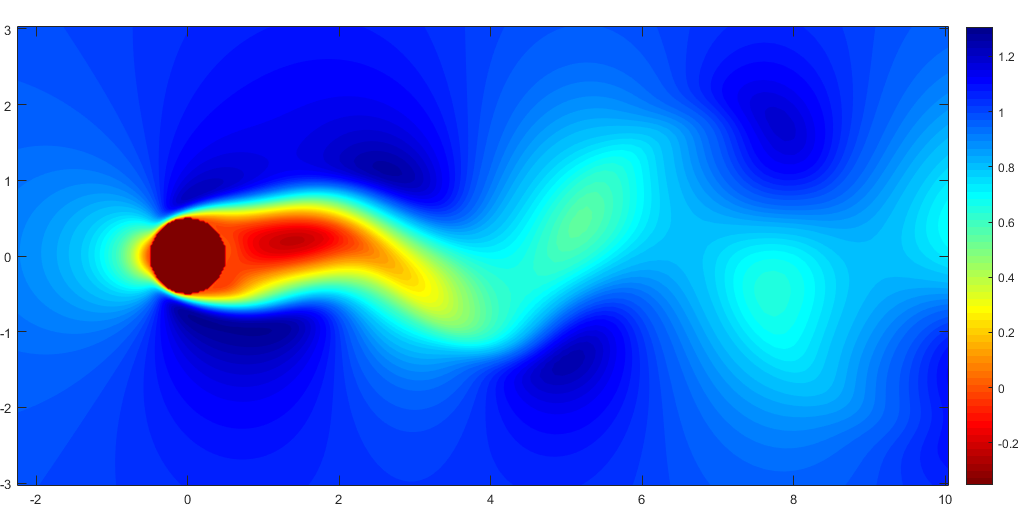
\includegraphics[width=0.23\textwidth]{snap100_0}		}
	\subfloat[Snapshot 10]{
		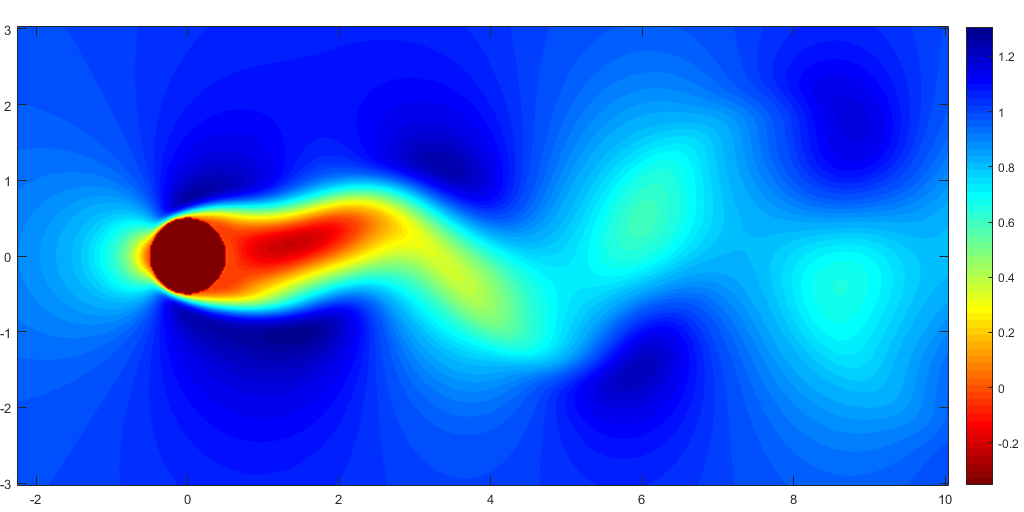
\includegraphics[width=0.23\textwidth]{snap100_10}		}
	\subfloat[Snapshot 20]{
		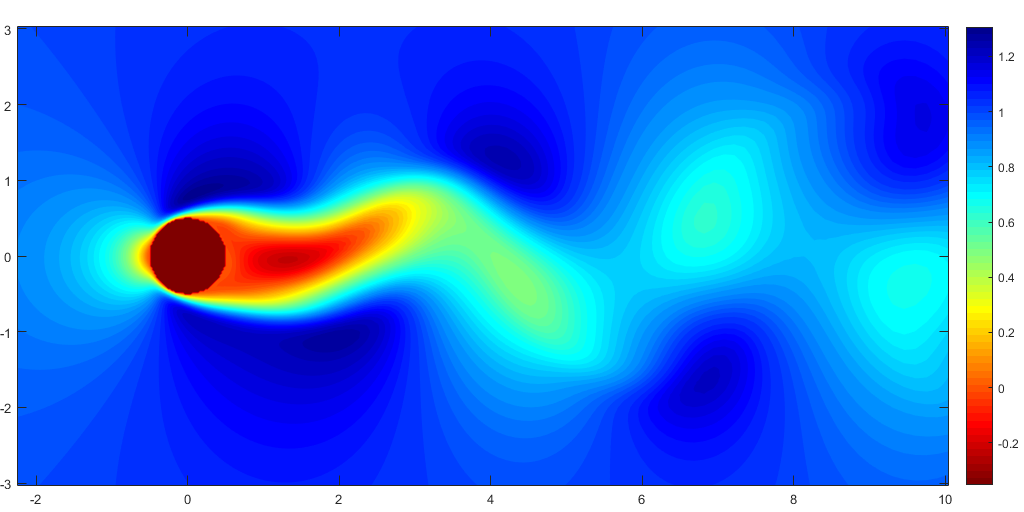
\includegraphics[width=0.23\textwidth]{snap100_20}		}
	\subfloat[Snapshot 30]{
		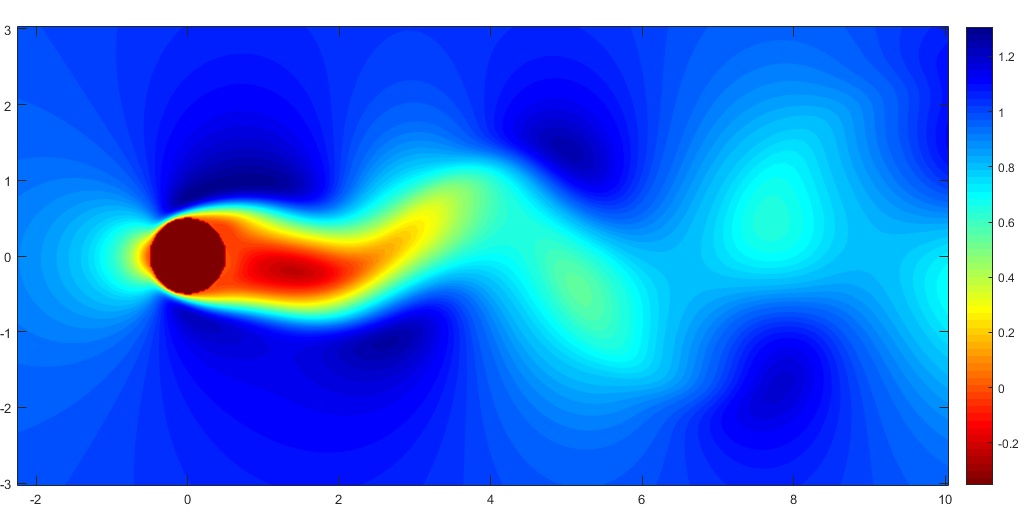
\includegraphics[width=0.23\textwidth]{snap100_30}		}\\
	\subfloat[Snapshot 0]{
		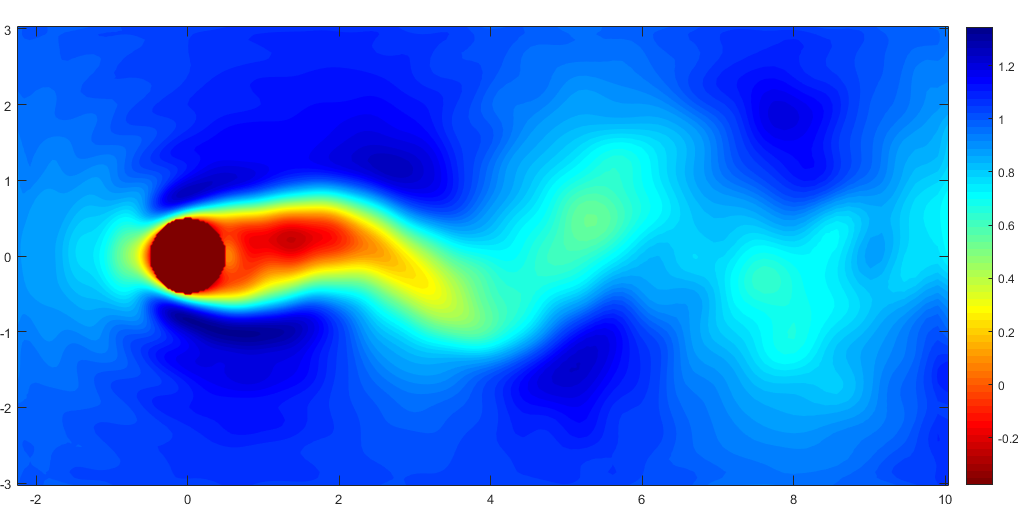
\includegraphics[width=0.23\textwidth]{snap100_c600_0}		}
	\subfloat[Snapshot 10]{
		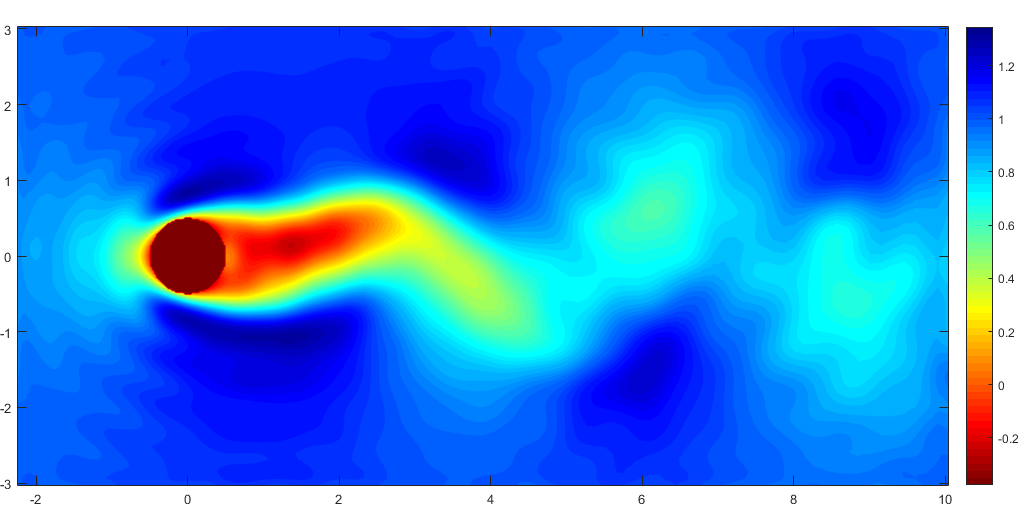
\includegraphics[width=0.23\textwidth]{snap100_c600_10}		}
	\subfloat[Snapshot 20]{
		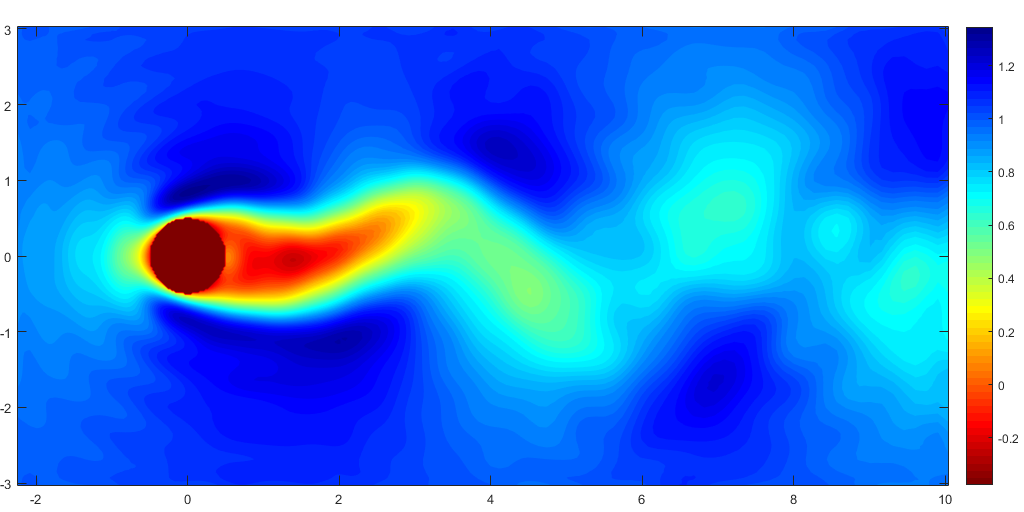
\includegraphics[width=0.23\textwidth]{snap100_c600_20}		}
	\subfloat[Snapshot 30]{
		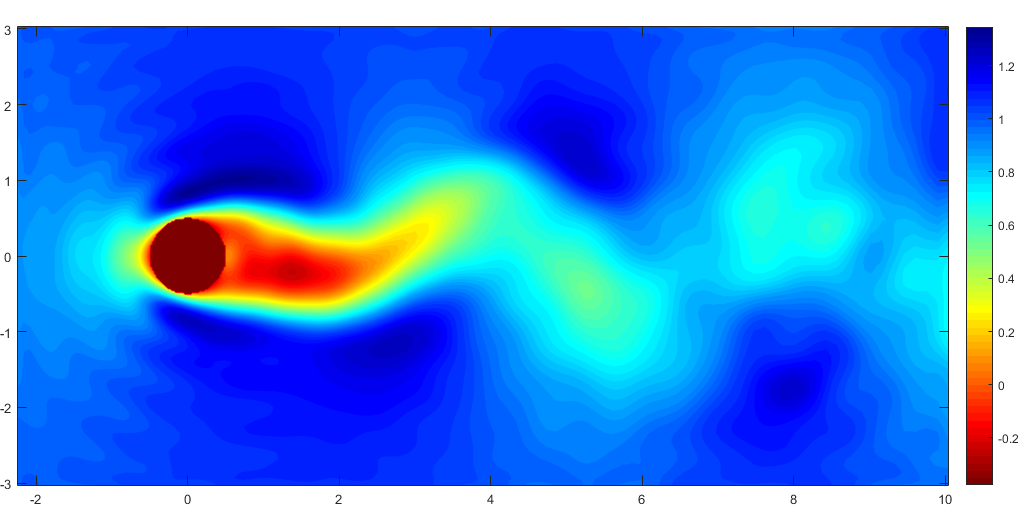
\includegraphics[width=0.23\textwidth]{snap100_c600_30}		}
	
	\caption{Visualization of Fluid Flow at Re = 100, CFD (a-d), E-GP (e-h)}
	\label{fig:cfd_100}
\end{figure*}

\begin{figure*}[h] %{r}{0.5\textwidth}
	\centering
	\subfloat[Snapshot 0]{
		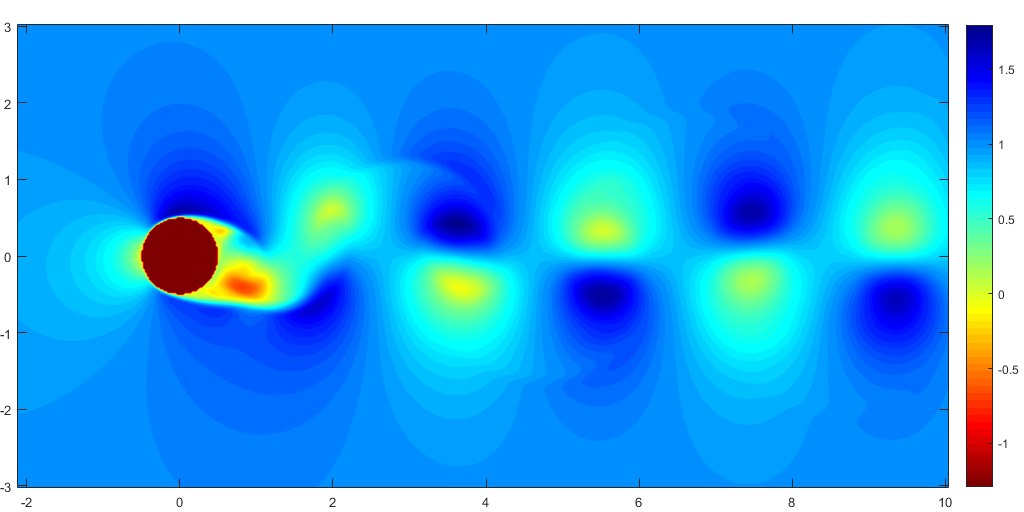
\includegraphics[width=0.23\textwidth]{snap1000_0}		}
	\subfloat[Snapshot 5]{
		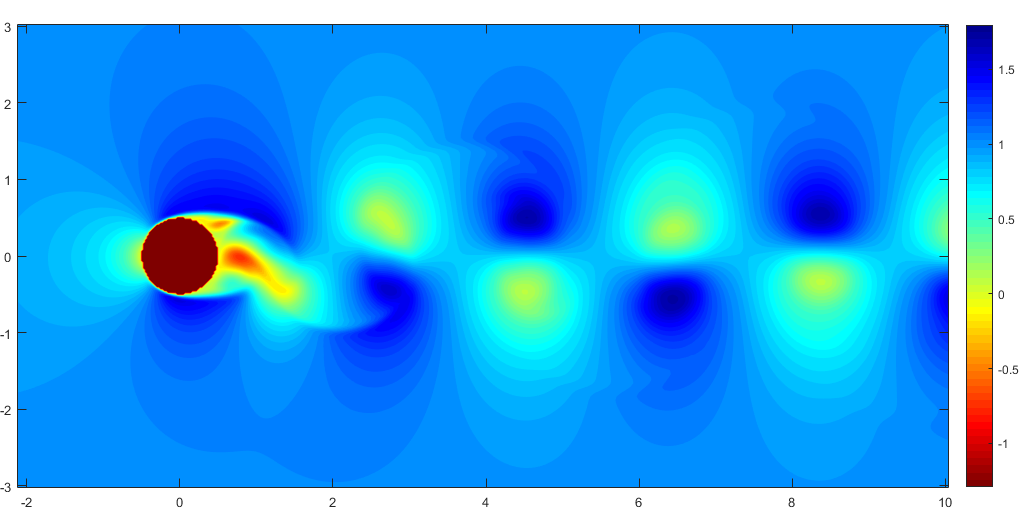
\includegraphics[width=0.23\textwidth]{snap1000_5}		}
	\subfloat[Snapshot 10]{
		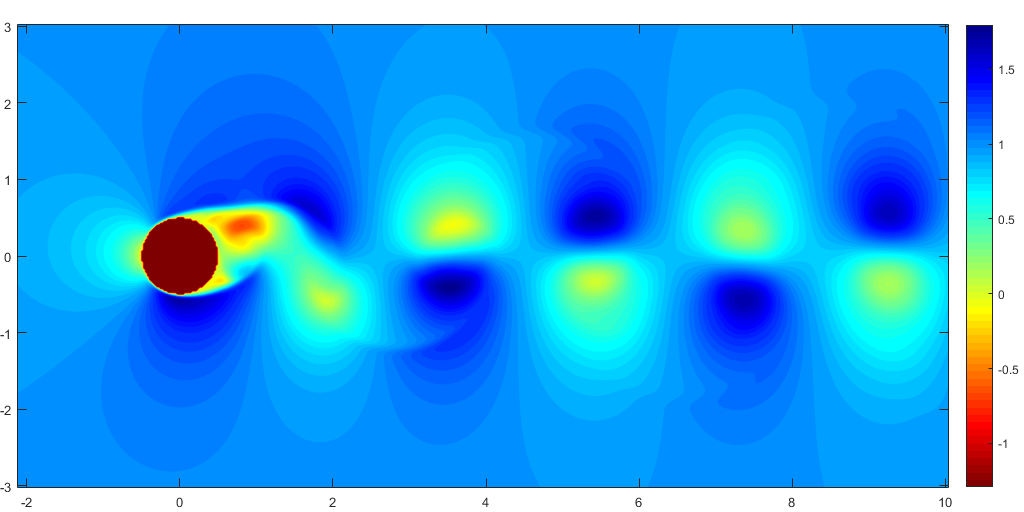
\includegraphics[width=0.23\textwidth]{snap1000_10}		}
	\subfloat[Snapshot 15]{
		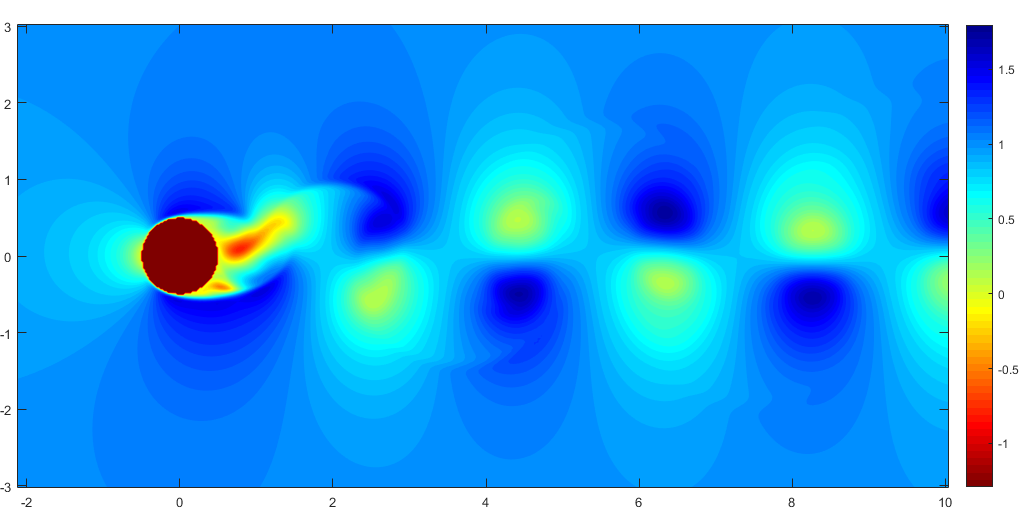
\includegraphics[width=0.24\textwidth]{snap1000_15}		}\\
	\subfloat[Snapshot 0]{
		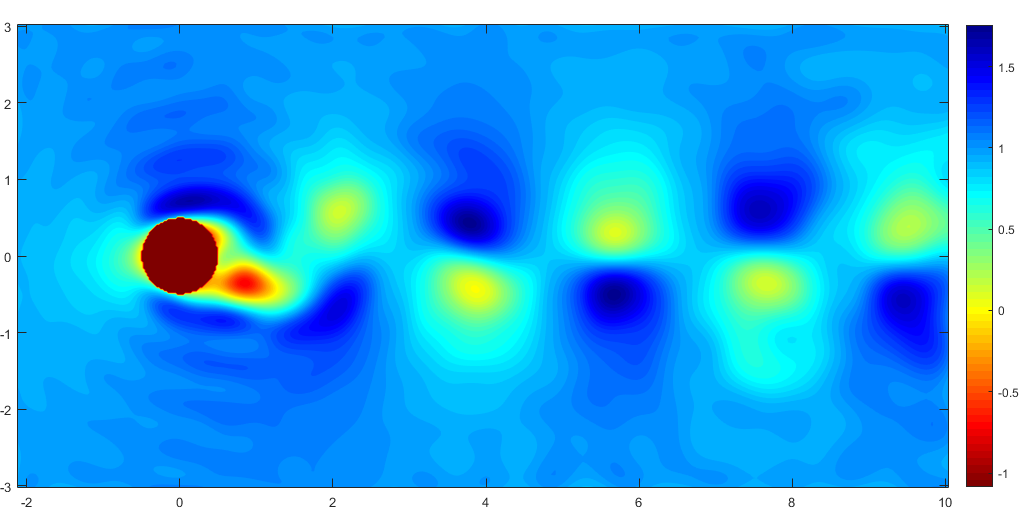
\includegraphics[width=0.24\textwidth]{snap1000_c600_0}		}
	\subfloat[Snapshot 5]{
		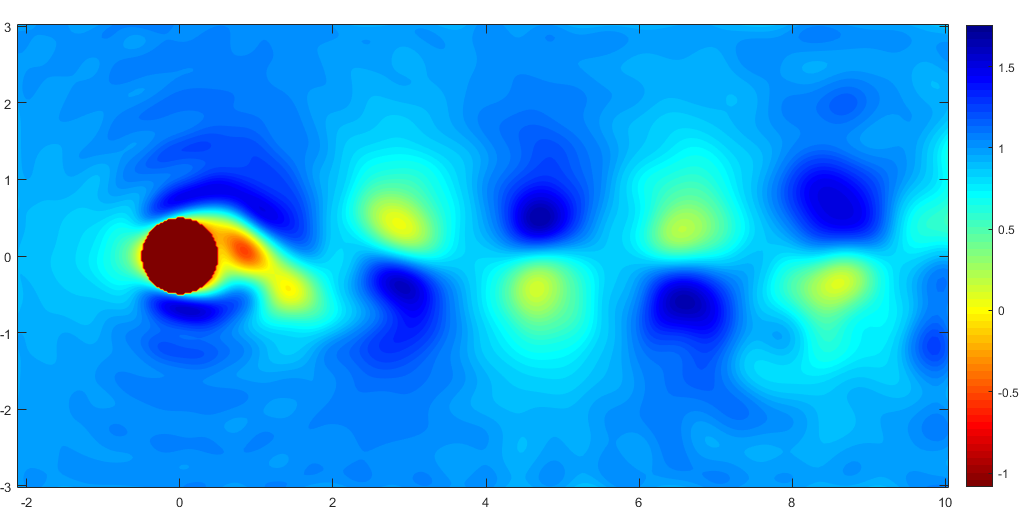
\includegraphics[width=0.23\textwidth]{snap1000_c600_5}		}
	\subfloat[Snapshot 10]{
		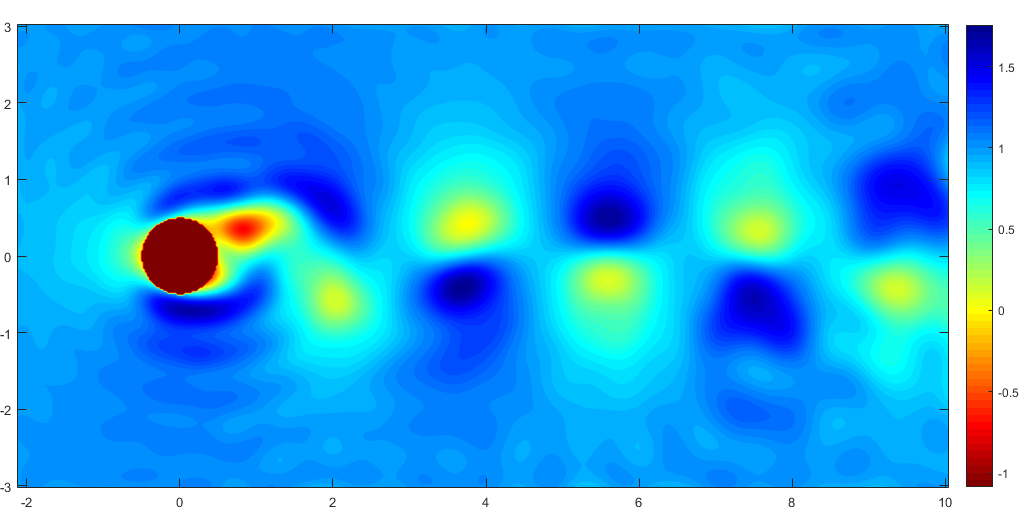
\includegraphics[width=0.23\textwidth]{snap1000_c600_10}	}
	\subfloat[Snapshot 15]{
		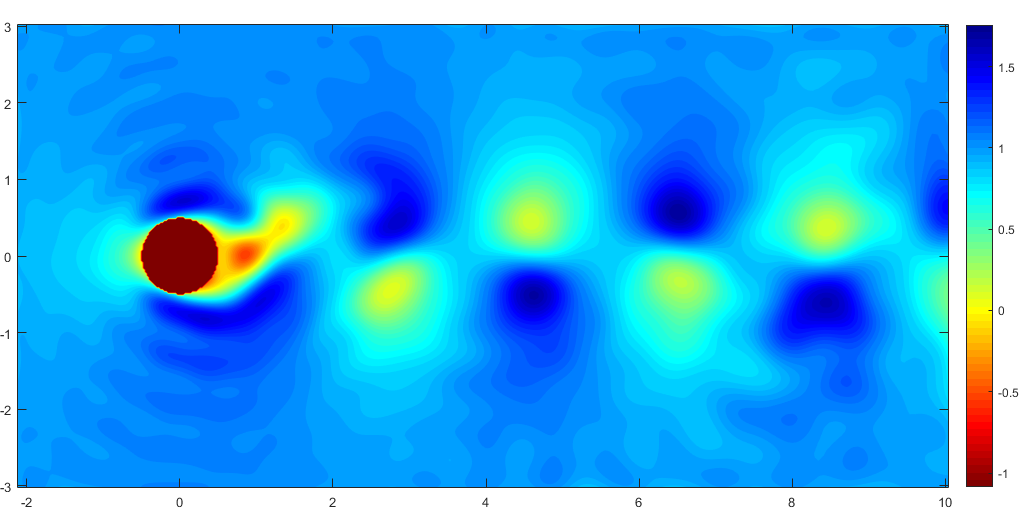
\includegraphics[width=0.23\textwidth]{snap1000_c600_15}	}
	\caption{Visualization of Fluid Flow at Re = 1000, CFD (a-d), E-GP (e-h)}
	\label{fig:cfd_1000}
\end{figure*}

We used the Gaussian RBF kernel $\kernel(x,y) = e^{-\|x-y\|^2/2\s^2}$ in our E-GP model, with $\s$ estimated to be 0.4. Using a budget of 600 kernel centers (see Figure \ref{fig:eigen100}-\ref{fig:eigen1000}, and note how they cluster in the most dynamic regions), we find a $600\times600$ matrix $\dualopApprox$ which accurately (Figure \ref{fig:errors}) captures the dynamics of the nonlinear system. We can use this to propagate single initial condition $\weight_{0}$ forward to make predictions, then compare the predictions to the original training data. We found total percentage errors between 3\% for Re=100 and 7-8\% for Re=1000, as can be seen in the solid lines in Figure \ref{fig:errors}. We define the total percentage errors as
$E_\tindex = \frac{\|y_\tindex-\bar y_\tindex\|_2}{\|\bar y_\tindex\|_2}$
where $\bar y_\tindex$ is the output vector for time $\tindex$ and $y_\tindex$ is the E-GP estimate at that time. Note that \emph{the size of the model has been reduced by almost two orders of magnitude} from the original CFD data. This process takes about 13 minutes in MATLAB for a 200 snapshot by 95,000 point set on an ordinary Intel i7 4.00 GHz processor.

\subsection{One Transition Matrix for Everything}\label{sec:lotr}

In order to approach the challenge of generalizing across similar spatiotemporally evolving systems, the first question we had to answer is whether we can find an $\dualopApprox$ matrix that accurately captures the dynamics of multiple similar flows. The answer to that question is \textit{yes}, using the trajectory concatenation method. Amazingly, a single model generated this way works almost as well on all five data sets as do five individual models trained on each data set separately. This is confirmed by both the total error plots (Figure \ref{fig:errors}), which show only slight increases in each of the total percentage error plots, and visual inspection of the dynamic modes displayed. This result is even more surprising in light of the fact that the rate of vortex shedding for each Reynolds number is different. By taking a Fourier transform of the time evolution of a data point located at (0.5,8), we find that for the original data sets the vortex shedding frequency is 0.448 Hz, 1.260 Hz, 1.380 Hz, 1.388, and 1.401 Hz for Re=100, 300, 600, 800, and 1000 respectively, and for the E-GP models the frequencies are 0.452 Hz, 1.21 Hz, 1.36 Hz, 1.36 Hz, and 1.36 Hz respectively.

\begin{figure*}[h] %{r}{0.5\textwidth}
	\centering
	\subfloat[\small{Universal Generalizer vs Individual Models}]{
		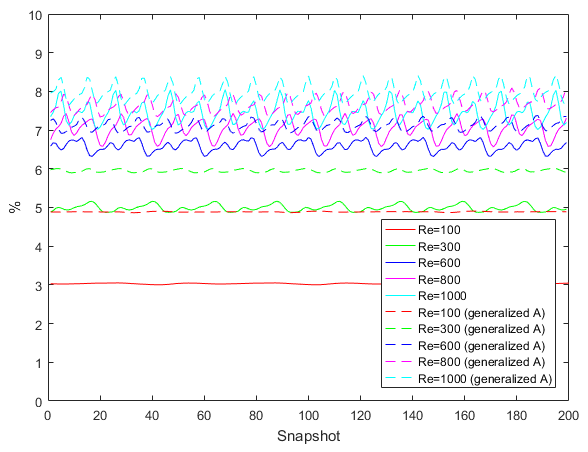
\includegraphics[width=0.38\textwidth]{errors}
		\label{fig:errors}		}
	\subfloat[\small{Different Models Tested on Re=800}]{
		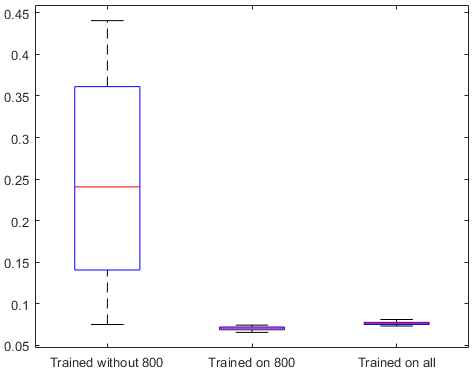
\includegraphics[width=0.36\textwidth]{boxploterrors800}
		\label{fig:errors_boxplot}		}
	\caption{Total Percentage Errors}
\end{figure*}

\subsection{Generalizing from Learned Dynamics to Unknown Dynamics}\label{sec:generalize}

Having seen that it is possible to find a single transition in the weight space that models the dynamics systems over a range of parameters, the next challenge is to be able to model flows with parameters that the model has not been trained on. We derived an $\dualopApprox$ matrix from the Re=100, 300, 600, and 1000 data sets and tested it against the Re=800 data set. The results are below in Figure \ref{fig:errors_boxplot}. For the first 120 snapshots, the total percentage error remains under 10\%, which is satisfactory. After this, however, the total percentage error curves upwards as the slight errors in the transition matrix compound. Over 800 snapshots, we found an average total percentage error of less than 25\%. %Taking a long-range view of the error plots, we found that they curve back downward again sinusoidally at snapshot 600, 35\% error. This indicates that the source of the divergence is likely due to a slight error in the speed of the vortices. This is confirmed by Fourier analysis as above, with the generalized model producing a wake frequency of 1.427 Hz in comparison to the actual frequency of 1.388 Hz, a 2.8\% difference. This small difference explains why the model is accurate for approximately the first 10 cycles before it begins to diverge.

\subsection{Linear Dynamical Layer Analysis \& Insights}\label{sec:analysis}
Due to the spatial encoding of the weights which the linear transition model operates on, we are able to analyze the dynamics and find physical insights into the process. We demonstrate two techniques: (1) using eigendecomosition of the transition matrix to discover the eigenfunctions and invariant subspaces of system, and (2) visualizing the most significant spatial interactions in the system.

\begin{figure*}[h] %{r}{0.5\textwidth}
	\centering
	\subfloat[\small{Re = 100, $\varepsilon$ = 0.005}]{
		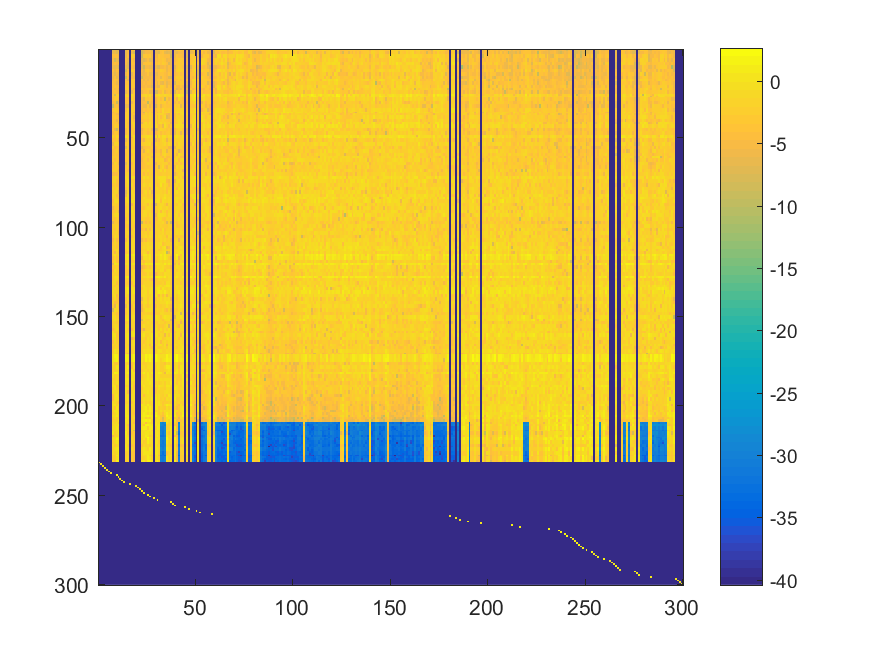
\includegraphics[width=0.31\textwidth]{matrix100floor5e3}
		\label{fig:eigen100}	}
	\subfloat[\small{Re = 1000, $\varepsilon$ = 0.05}]{
		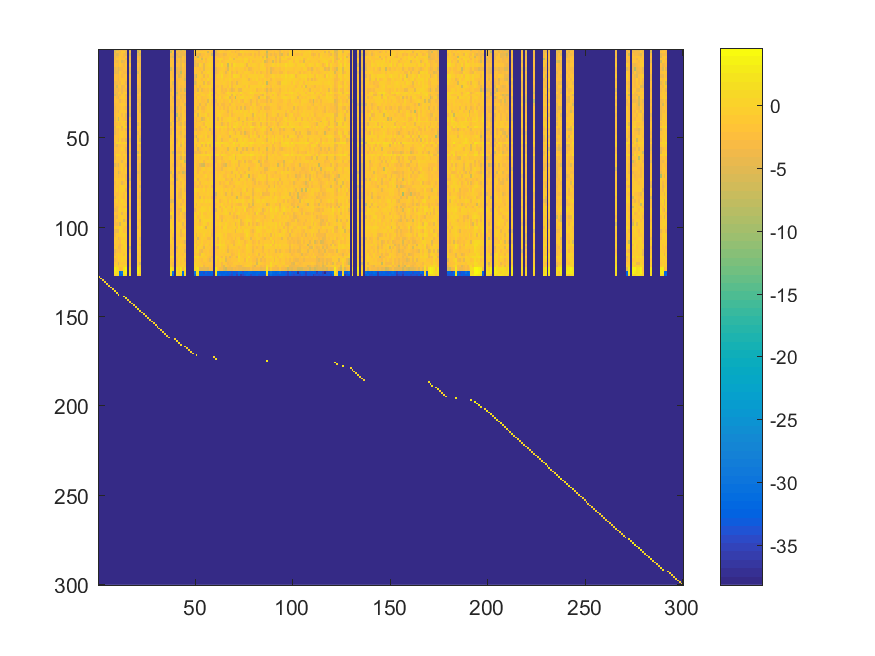
\includegraphics[width=0.31\textwidth]{matrix1000floor50e3}
		\label{fig:eigen1000}		}
	\subfloat[\small{All Reynolds numbers, $\varepsilon$ =0.069}]{
		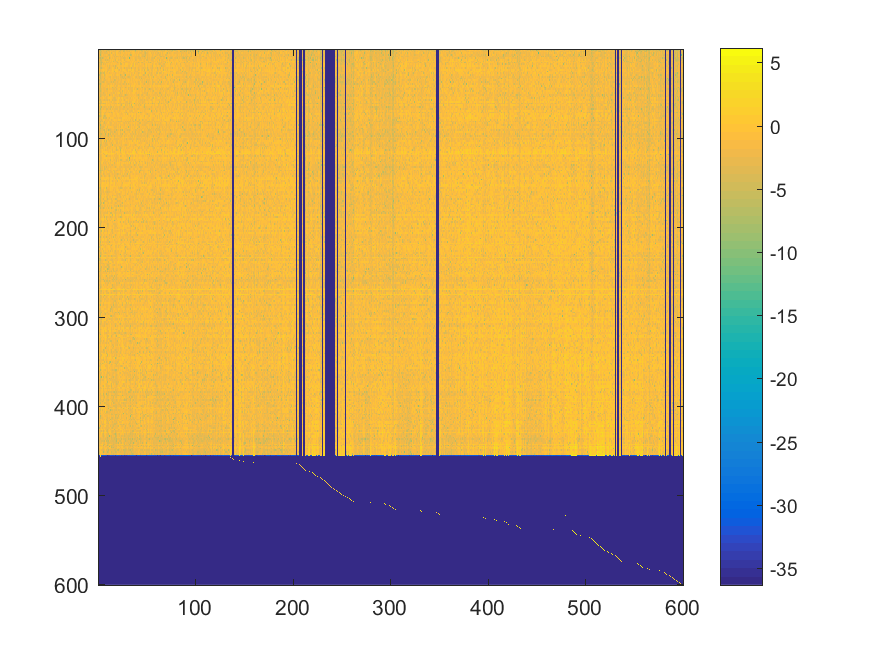
\includegraphics[width=0.31\textwidth]{matrixallfloor69}
		\label{fig:eigenall}	}
	\caption{Eigenvector Heat Maps}
\end{figure*}

An invariant subspace of a linear operator is a subspace of the Hilbert space such that any vector in the subspace remains in the subspace under transformation by the operator. By marking which kernel centers are associated with different subspaces, we can spatially separate the space into multiple dynamic modules. The physical insight is some areas of the space are dynamically entangled with each other, and other are independent of each other. For those interested in monitoring spatiotemporally evolving systems, the number and location of the invariant subspaces determines how many and where feedback sensors ought to be for robust prediction of the weights.

Before doing the Jordan decomposition of $\dualopApprox$, we zero any elements smaller than some small $\varepsilon$ in order to stabilize the algorithm for matrices with many elements close to zero. Afterwards we visualize the eigenvector matrix using a \emph{logarithmic} color chart, as seen in Figures \ref{fig:eigen100},\ref{fig:eigen1000},\ref{fig:eigenall}. These plots are for models trained individually on Re=100 and Re=1000 with 300 kernels, and on all five with 600 kernels, for comparison. We see three categories of eigenvector in the rows: (1) Rows at the bottom that have exactly one non-zero elements, (2) In the middle, a couple rows with a dozen significant elements, and (3) at the top a number of rows that affect the majority of the kernel centers in the space.

Each eigenvector of (1) spans its own invariant subspace, and is depicted in magenta circles in Figures \ref{fig:subspace100},\ref{fig:subspace1000},\ref{fig:subspaceall}. Category (3) is one invariant subspace, depicted with black crosses. Category (2) is subsumed in Category (3). The figures show that the dynamics near/around the cylinder and in its wake are so entangled that a single sensor measurement in that area may be sufficient to estimate over that entire subspace. On the other hand, areas far from the core of dynamic excitement are their own independent, invariant subspaces, and thus must be monitored locally.

Another way to visualize the operation of the linear transition matrix is to plot lines between kernel centers that are influencing each other strongly. That is, if we draw a line center $c_j$ to $c_i$ for each of the (relatively) largest elements $a_{ij}$ of $\dualopApprox$, one can see how the system dynamics are coupled spatially (Figures \ref{fig:haystack100},\ref{fig:haystack1000},\ref{fig:haystackall}). We can also plot the magnitude of $a_ij$ in a third axis for further insight into the most dominant dynamic connection in the system.

\begin{figure*}[h] %{r}{0.5\textwidth}
	\centering
	\subfloat[\small{Re = 100, $\varepsilon$ = 0.005}]{
		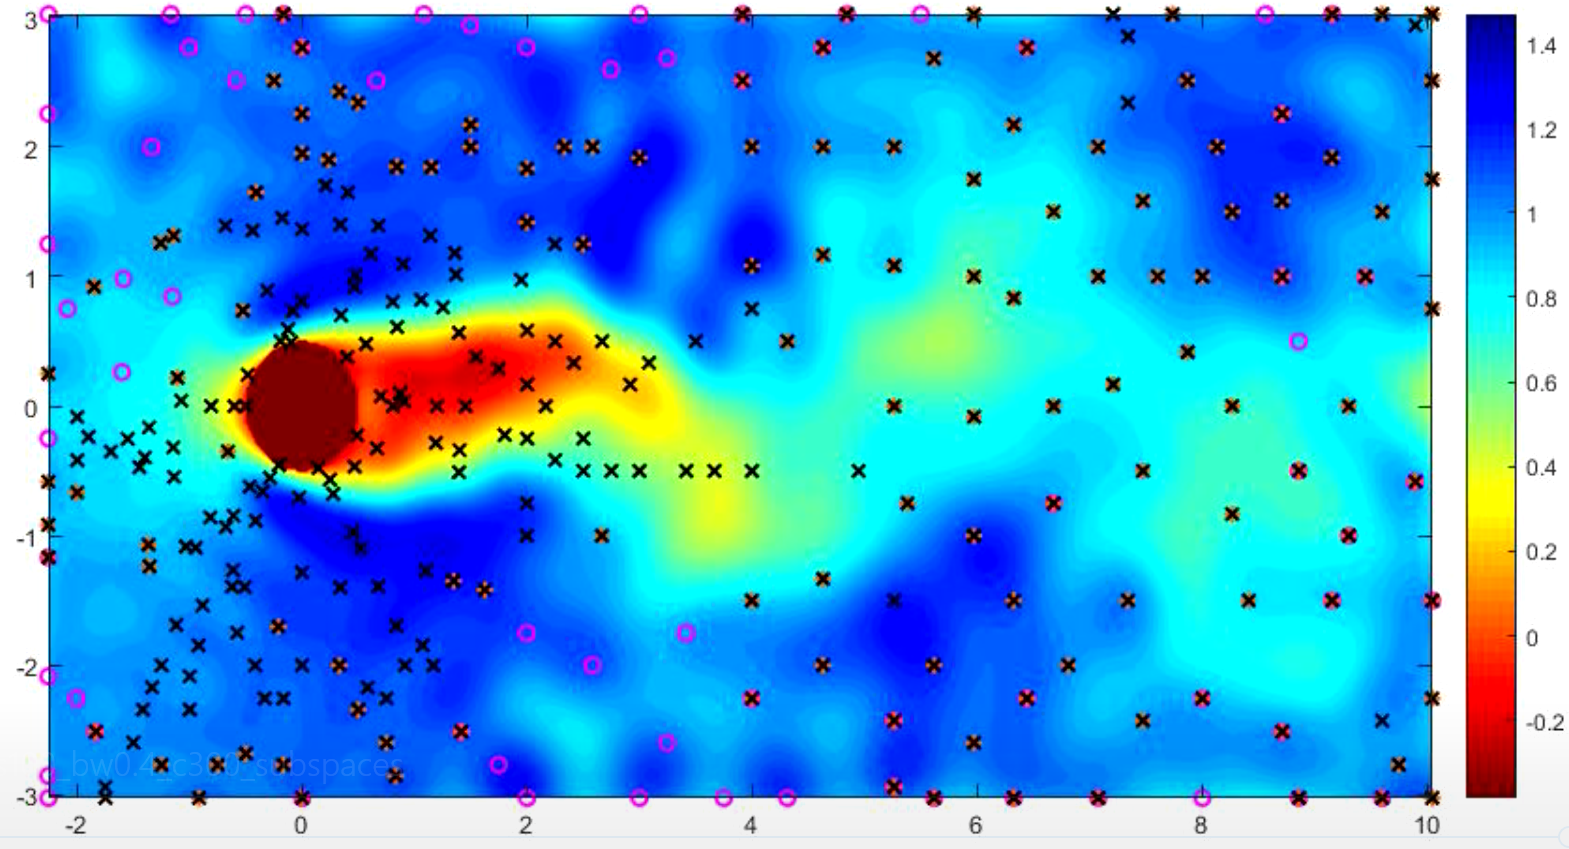
\includegraphics[width=0.30\textwidth]{subspaces100}
		\label{fig:subspace100}	}
	\subfloat[\small{Re = 1000, $\varepsilon$ = 0.05}]{
		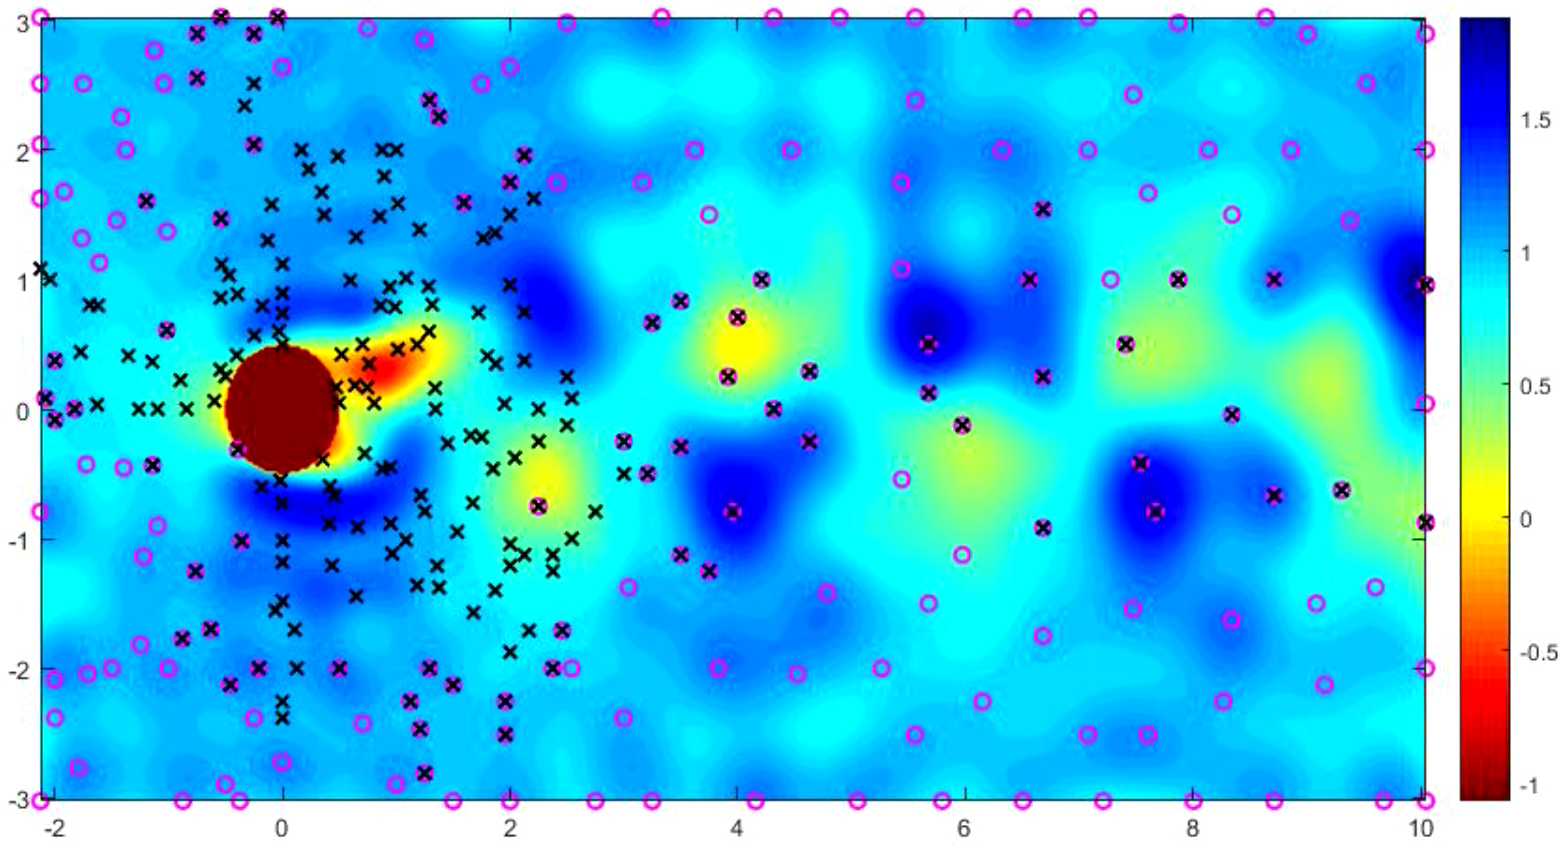
\includegraphics[width=0.30\textwidth]{subspaces1000}
		\label{fig:subspace1000}		}
	\subfloat[\small{All Reynolds numbers, $\varepsilon$ = 0.069}]{
		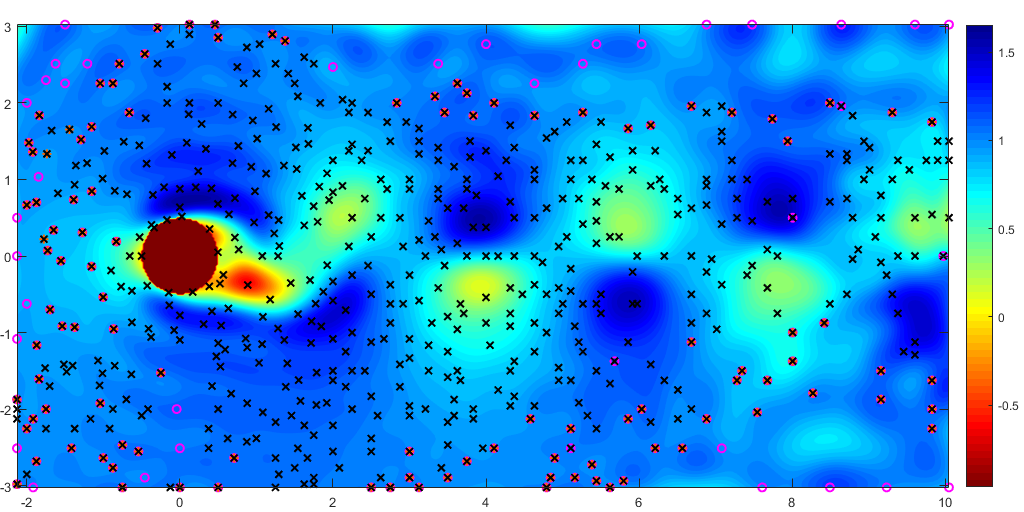
\includegraphics[width=0.34\textwidth]{subspacesall}
		\label{fig:subspaceall}	}
	\caption{Invariant Subspaces}
\end{figure*}


\begin{figure}[h] %{r}{0.5\textwidth}
	\centering
	\subfloat[\small{Re=100}]{
		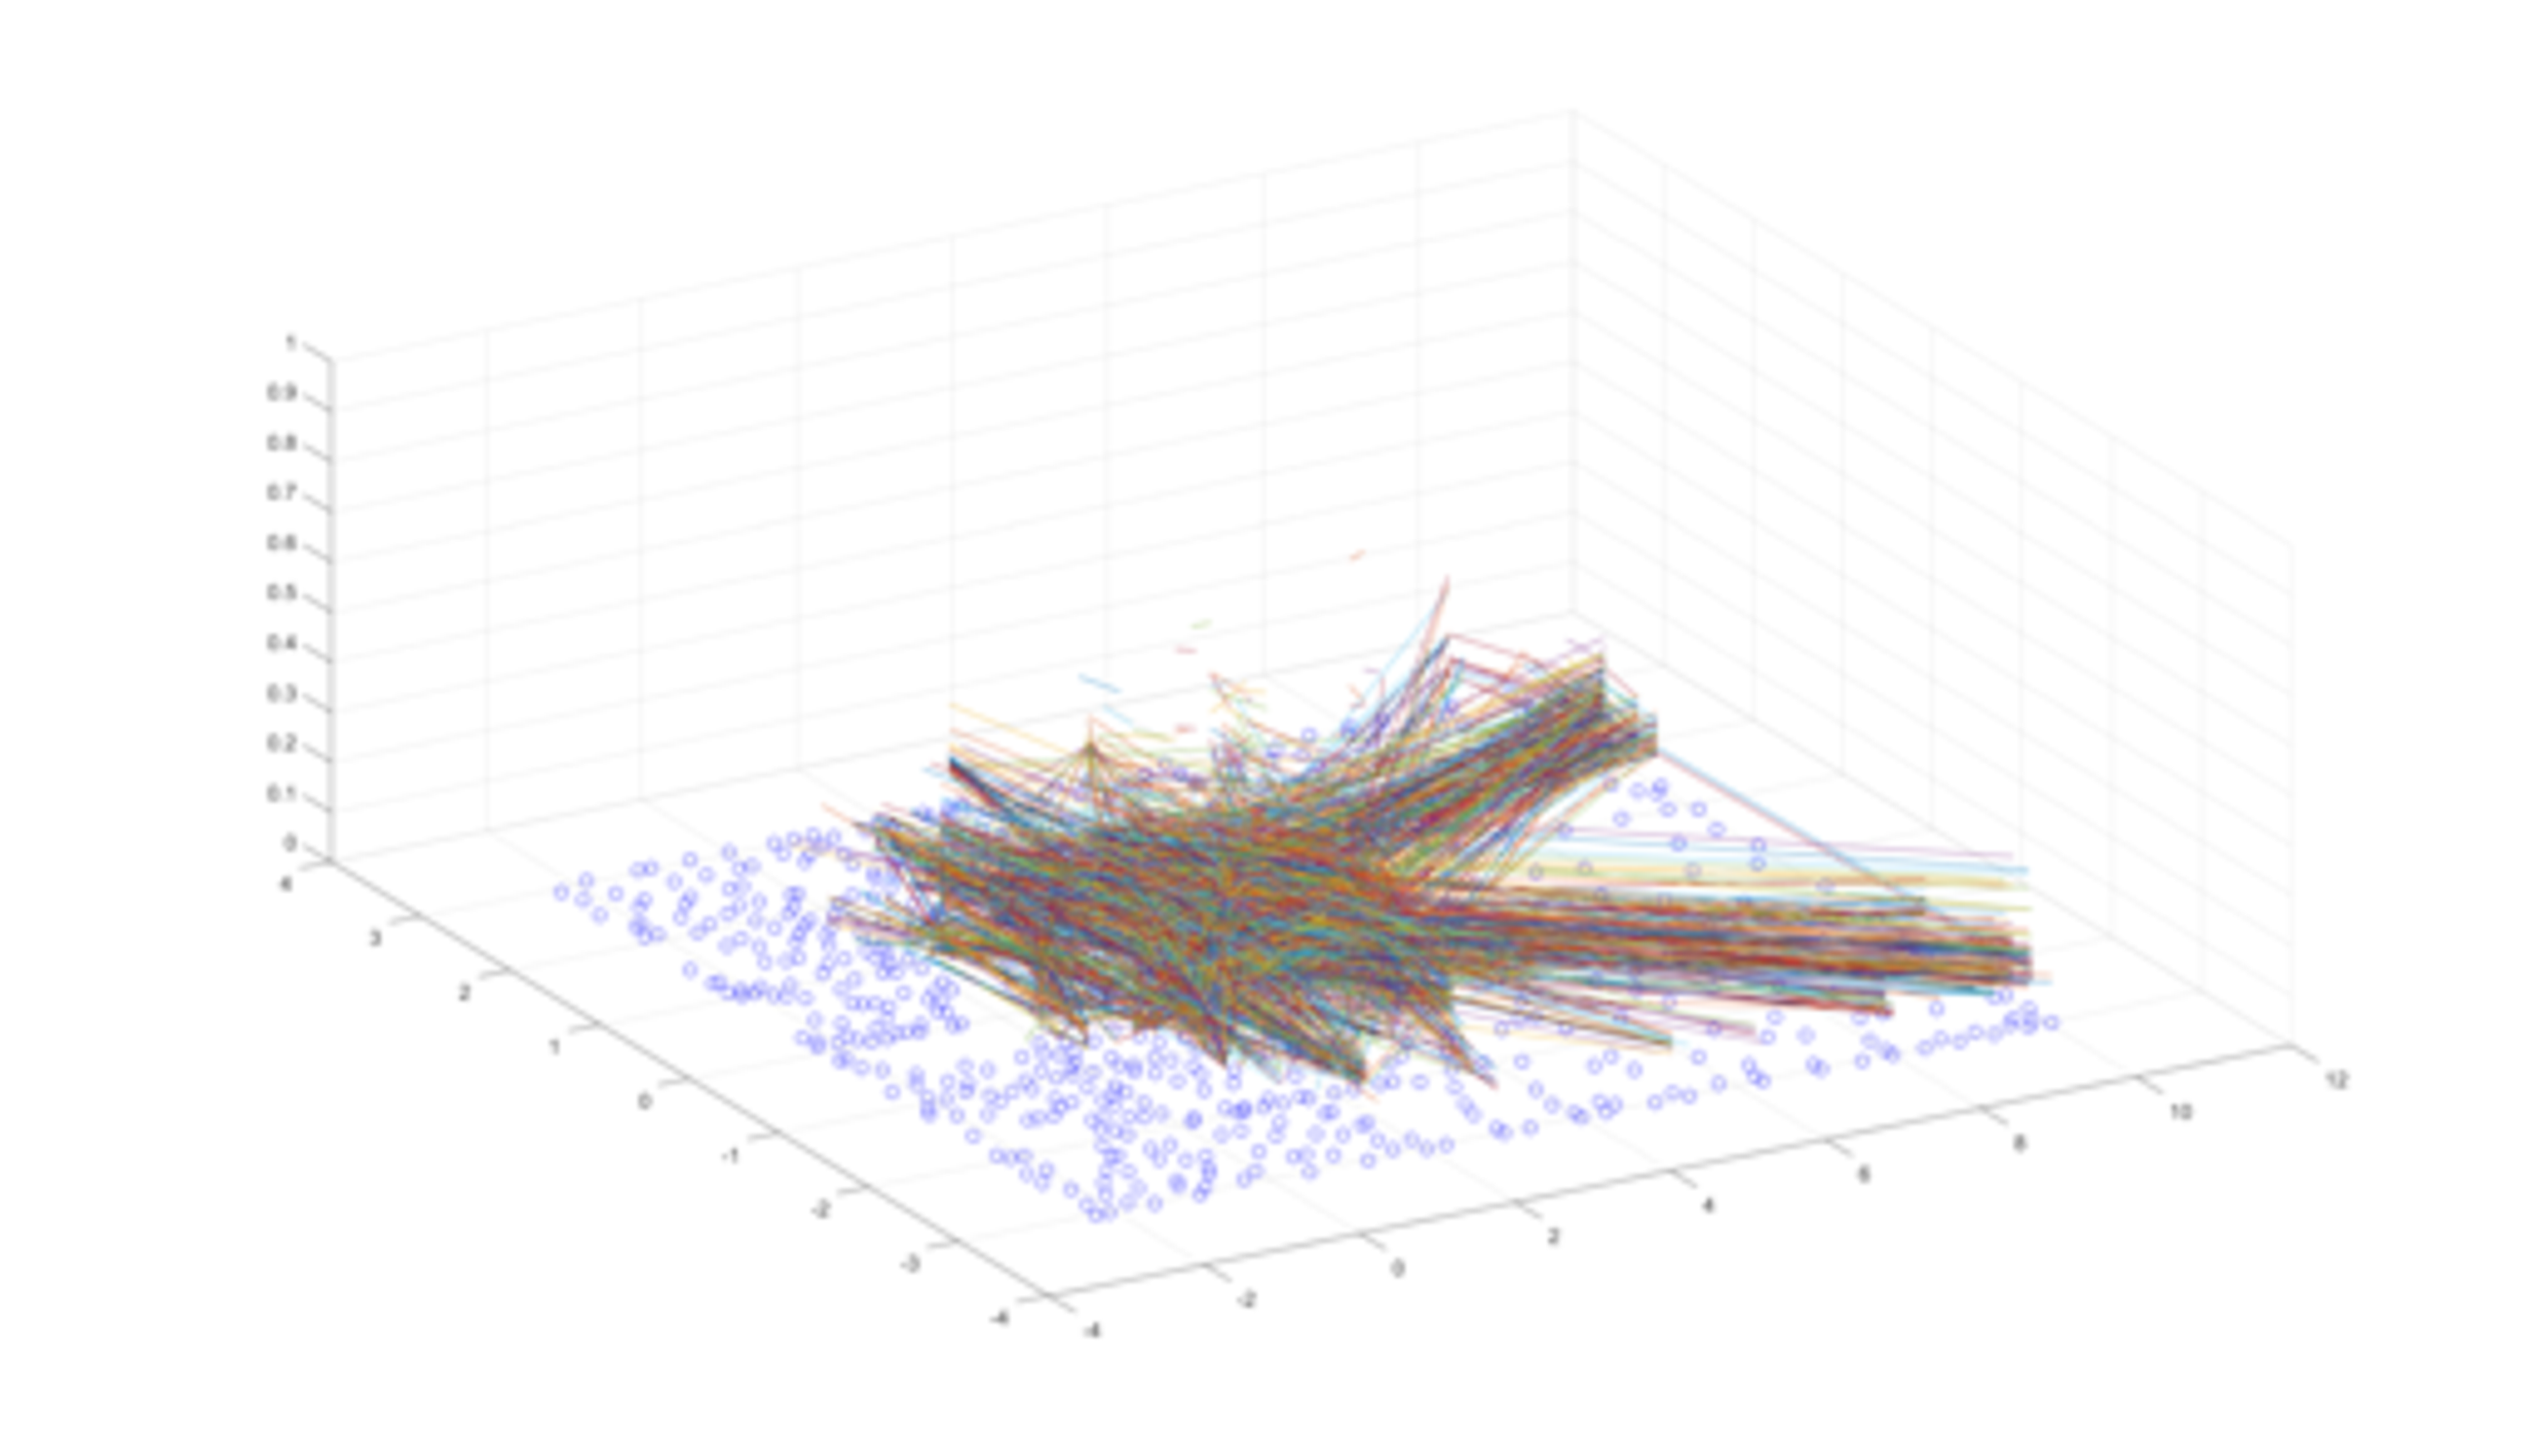
\includegraphics[width=0.31\textwidth]{Amatrix3d100}
		\label{fig:haystack100}	}
	\subfloat[\small{Re=1000}]{
		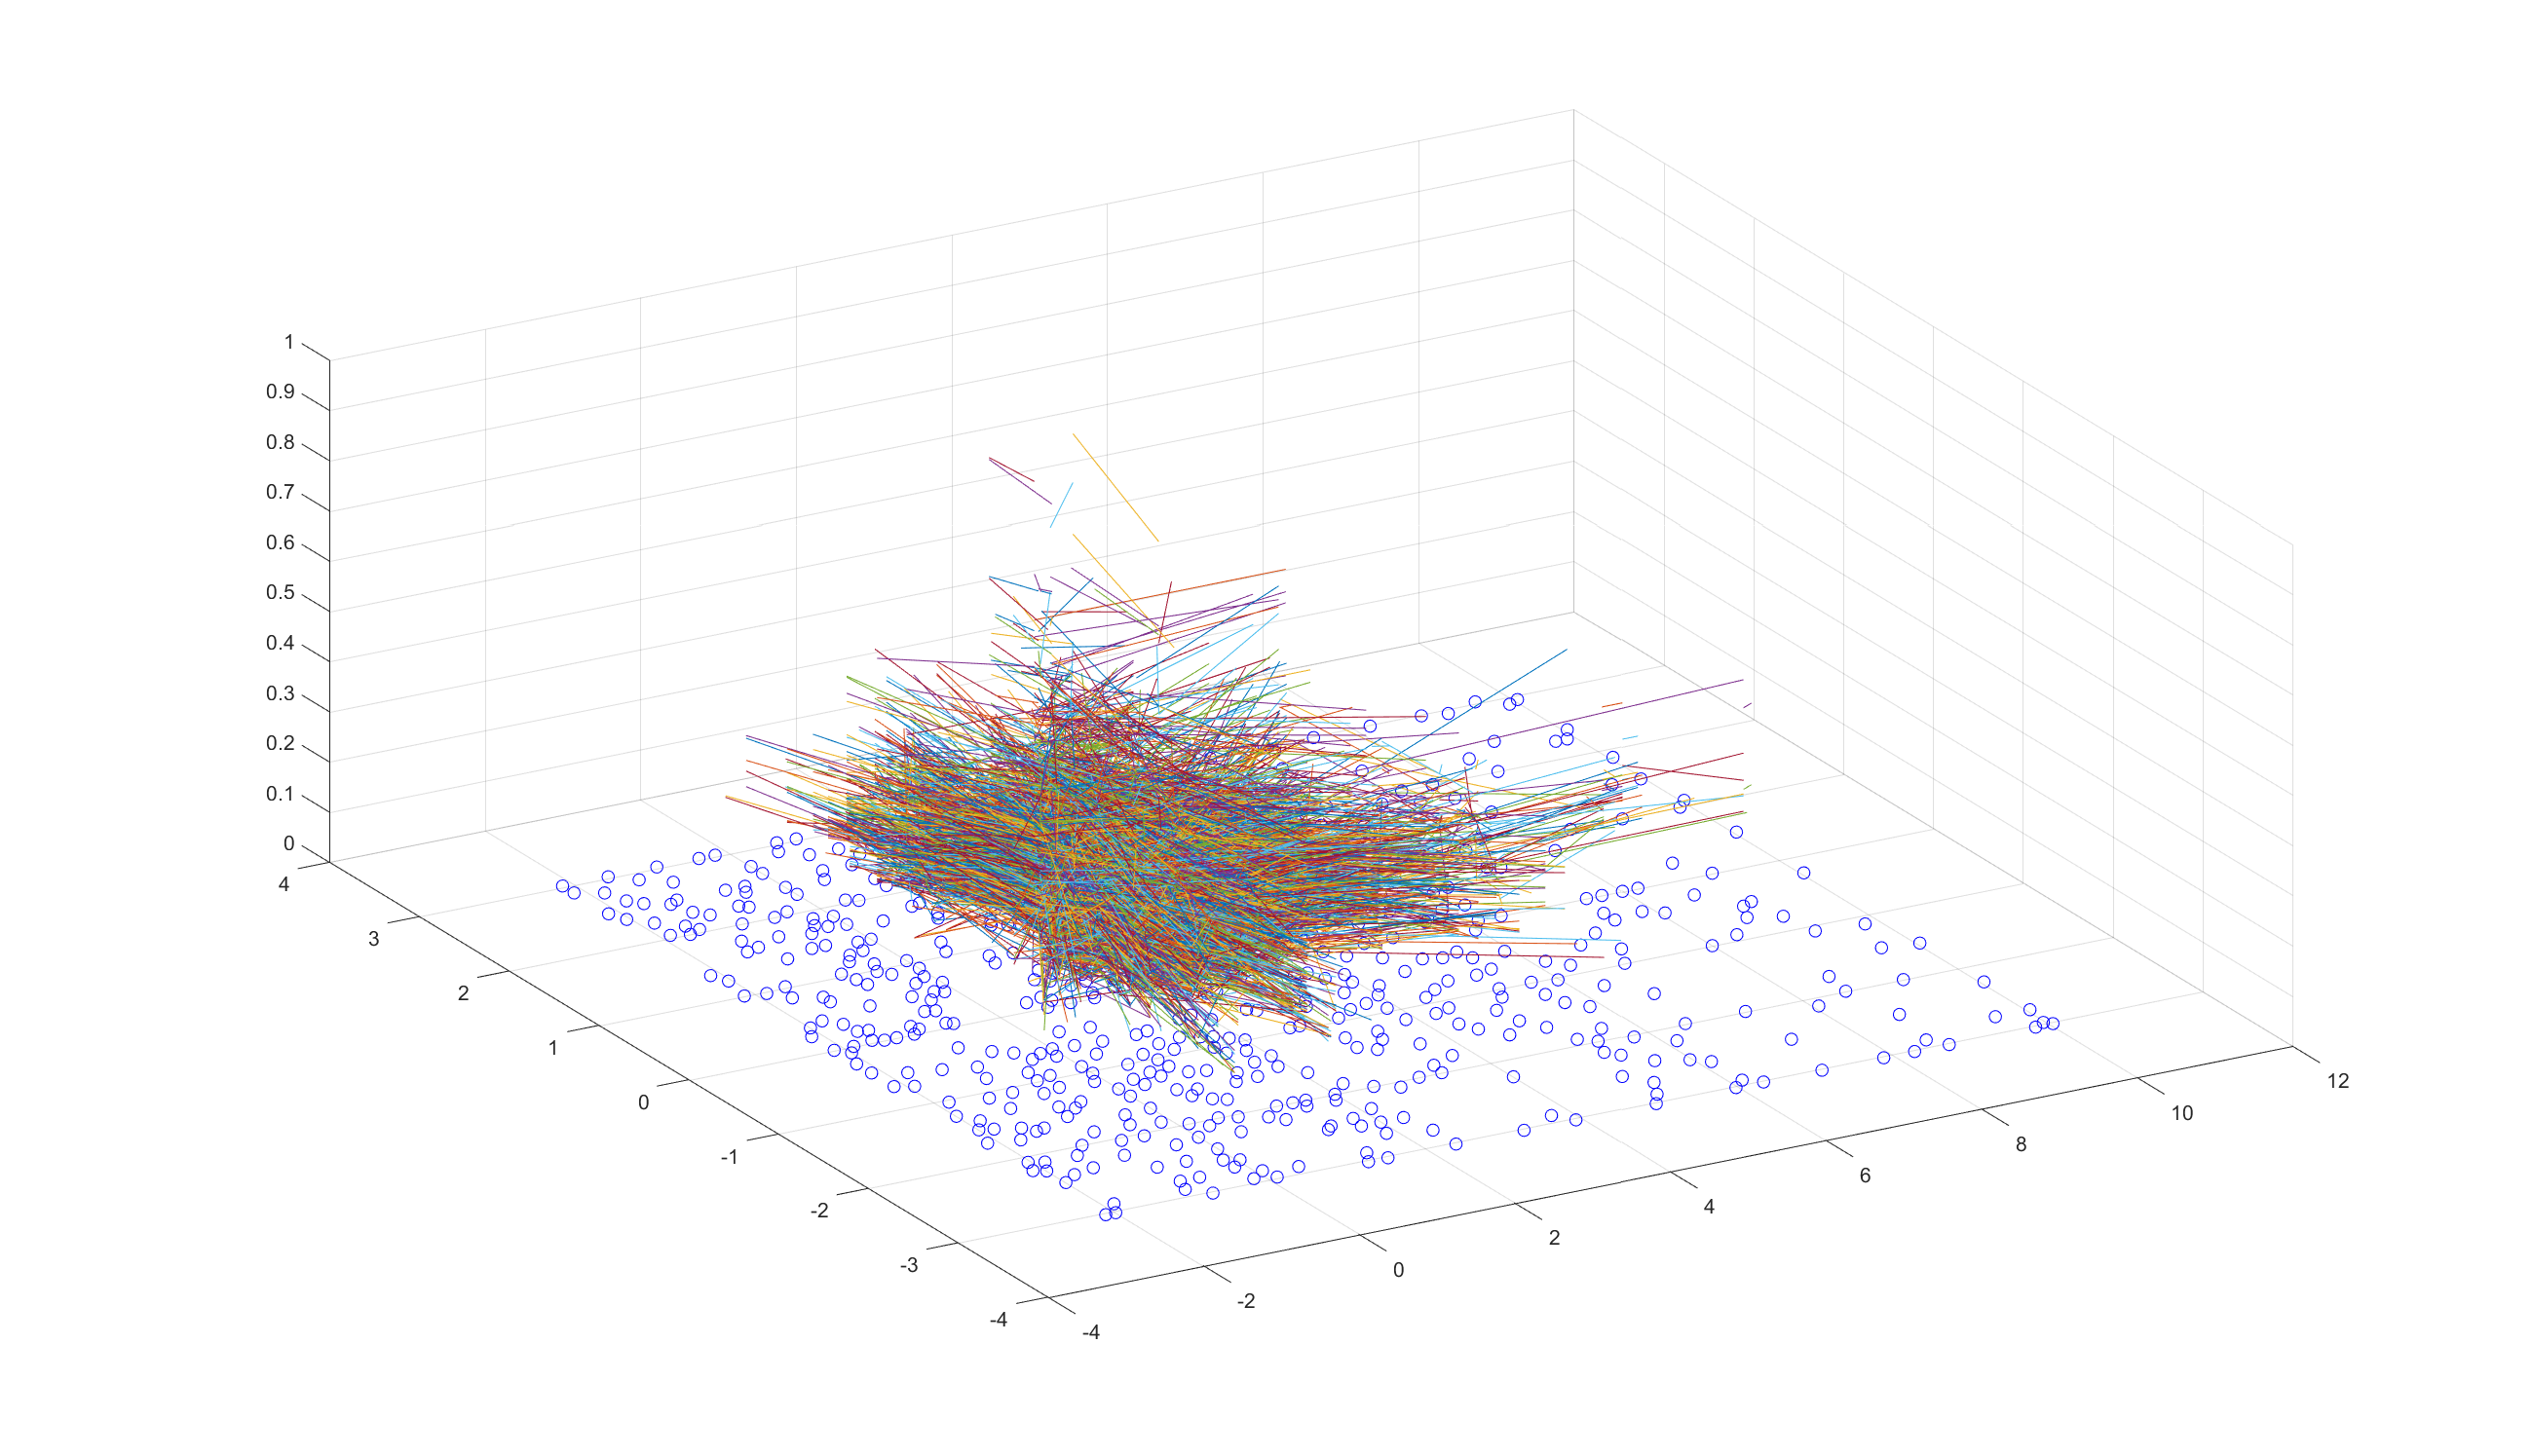
\includegraphics[width=0.31\textwidth]{Amatrix3d1000}
		\label{fig:haystack1000} }
	\subfloat[\small{Trained on all 5 data sets}]{
		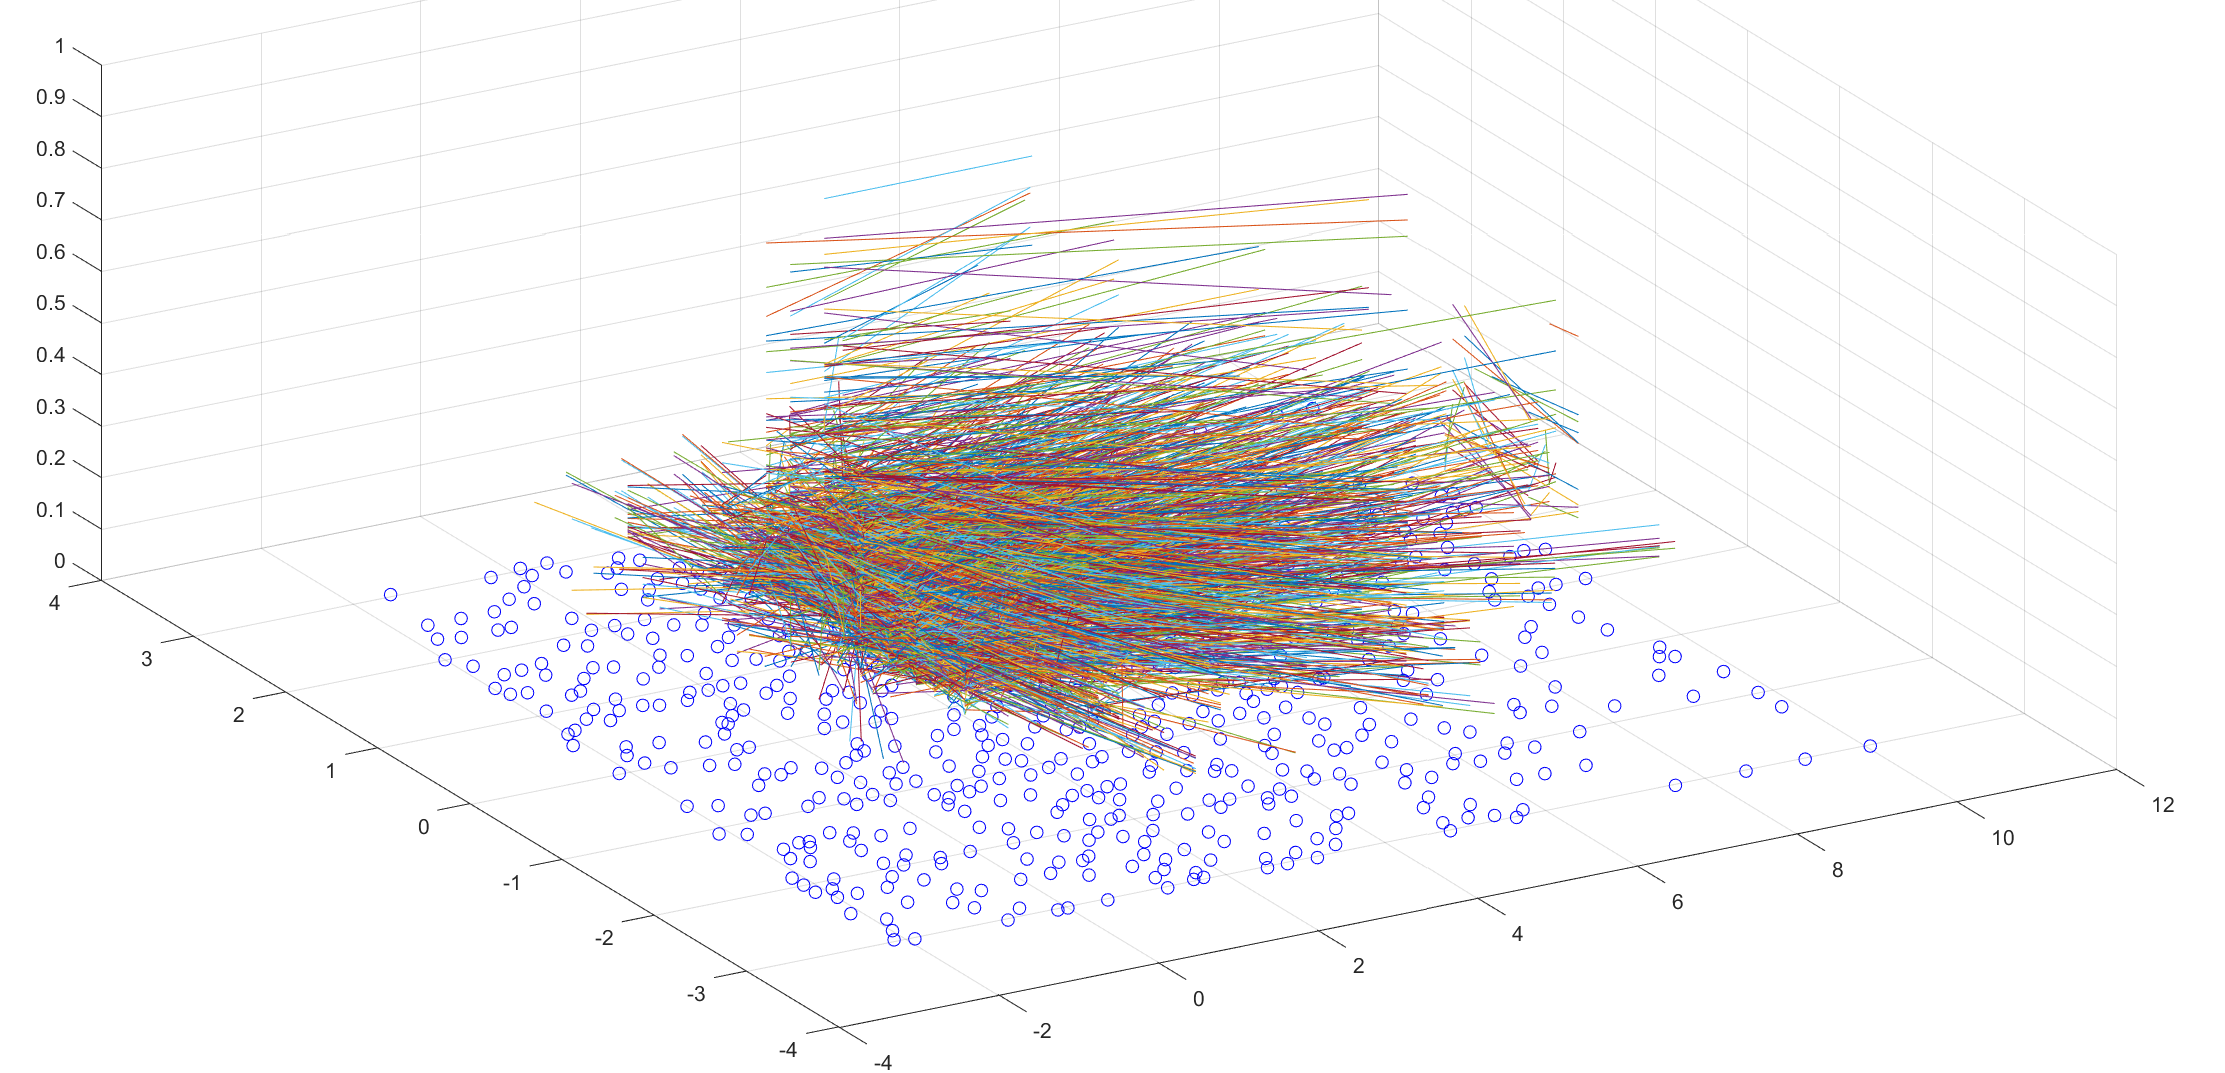
\includegraphics[width=0.31\textwidth]{Amatrix3dall}
		\label{fig:haystackall}	}
	\caption{Visualization of Co-Relations in Transition Matrix}
\end{figure}



%\begin{figure}[t]
%	\centering
%	\subfloat[\small{Gaussian}]{
%		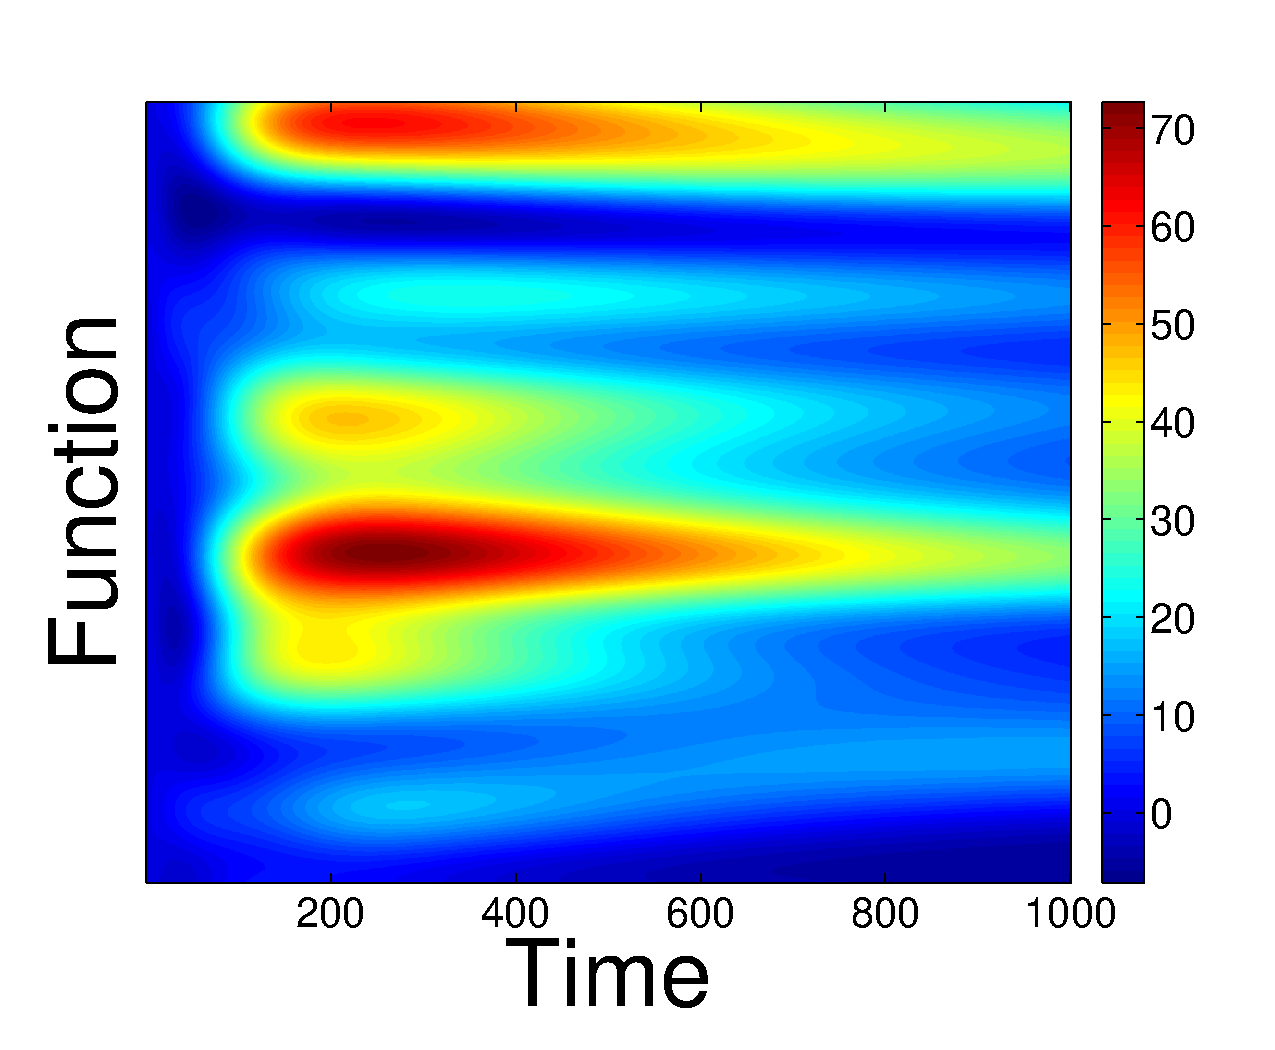
\includegraphics[width=0.25\columnwidth]{figures/kernel_evol_gaussian.pdf}
%	}
%	\subfloat[\small{Laplacian}]{
%		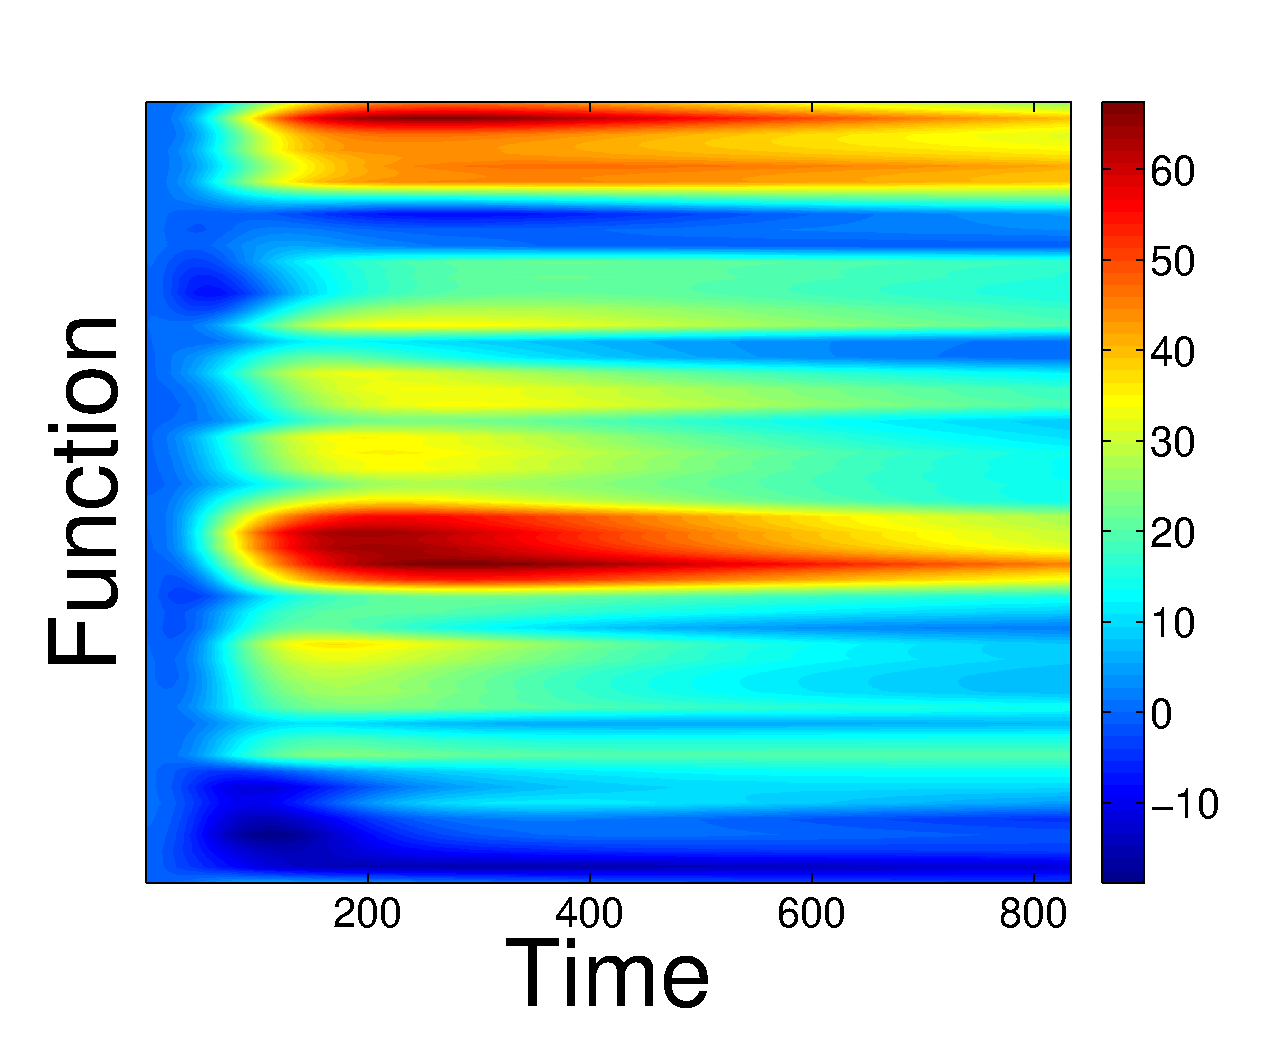
\includegraphics[width=0.25\columnwidth]{figures/kernel_evol_laplacian.pdf}
%	}
%	% \\
%	\subfloat[\small{Periodic}]{
%		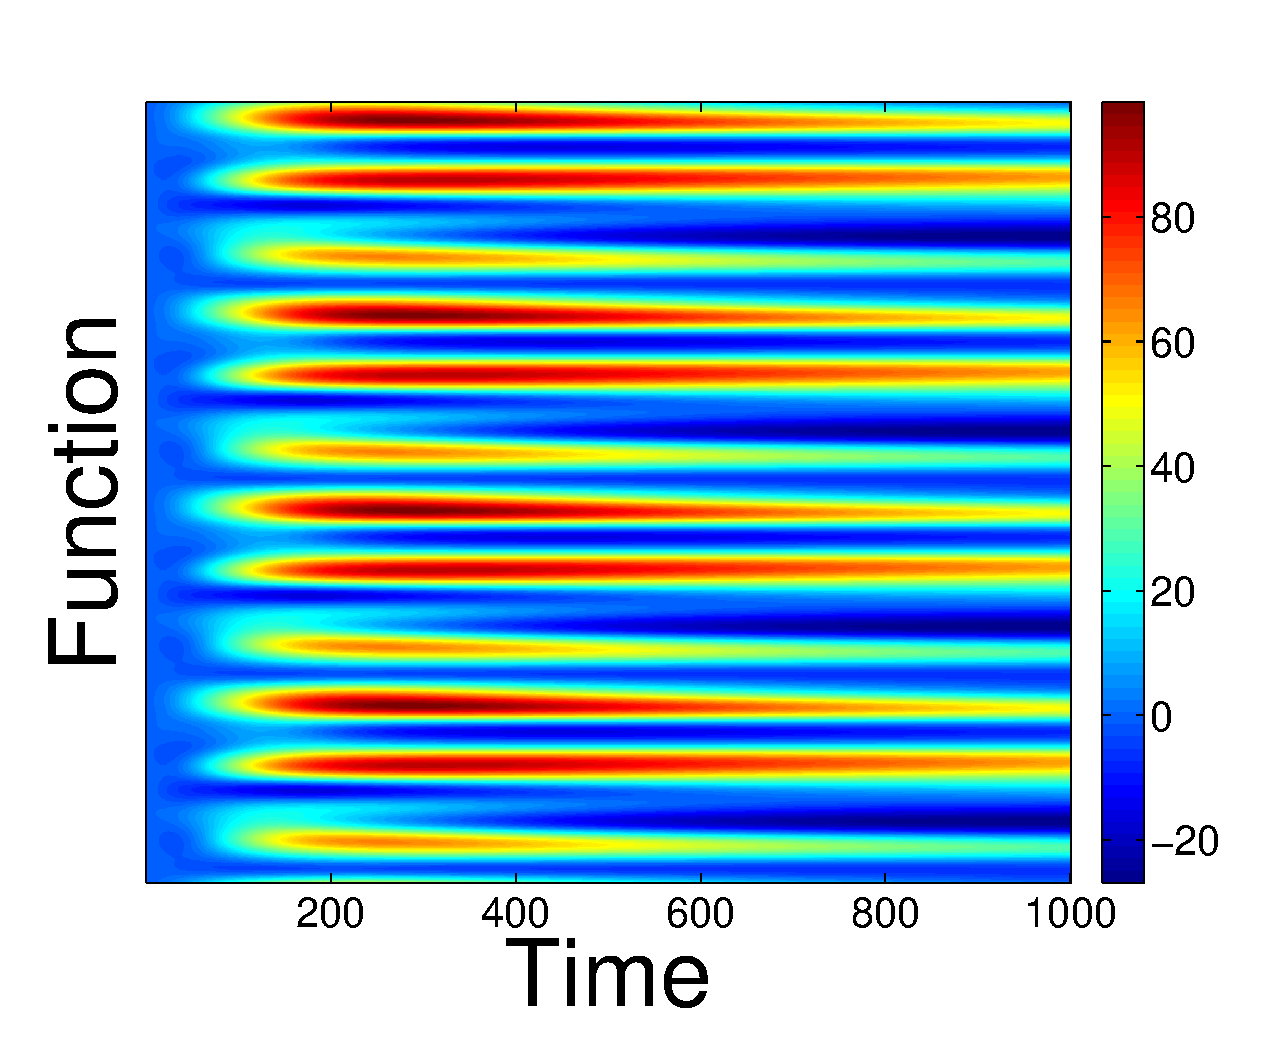
\includegraphics[width=0.25\columnwidth]{figures/kernel_evol_periodic.pdf}
%	}
%	% \subfloat[\small{Locally periodic}]{
%	%   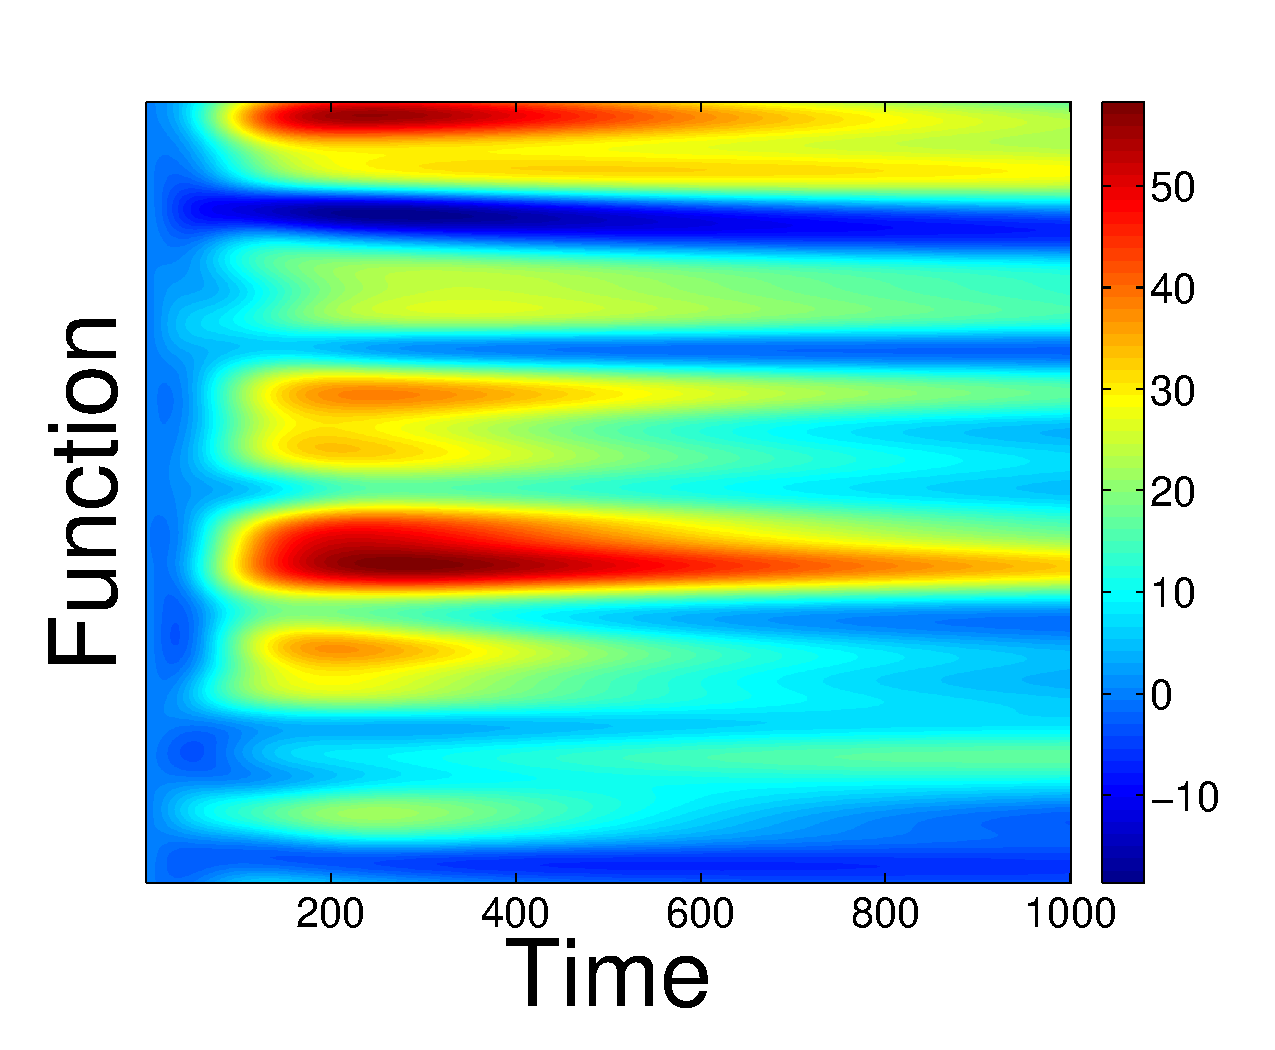
\includegraphics[width=0.3\columnwidth]{figures/kernel_evol_locally_periodic.pdf}
%	%}
%	\caption{\small{One-dimensional function evolution over a fixed transition matrix $A$, 
%			initial condition $\weight_0$ and centers $\shCent$, but with different kernels $\kernel(x,y)$. 
%			Each $y$-vector at a given value of $x$ represents the output of the function, which evolves from left to right. 
%			As seen, changing the kernel creates quite different dynamic behaviors. }%behavior for the same system.}
%	}
%	\label{fig:kernel_variation}
%\end{figure}




%\begin{figure}\label{fig:linsep}
%\centering
%    \subfloat[Data from classes $A$ and $B$.]
%    {
%    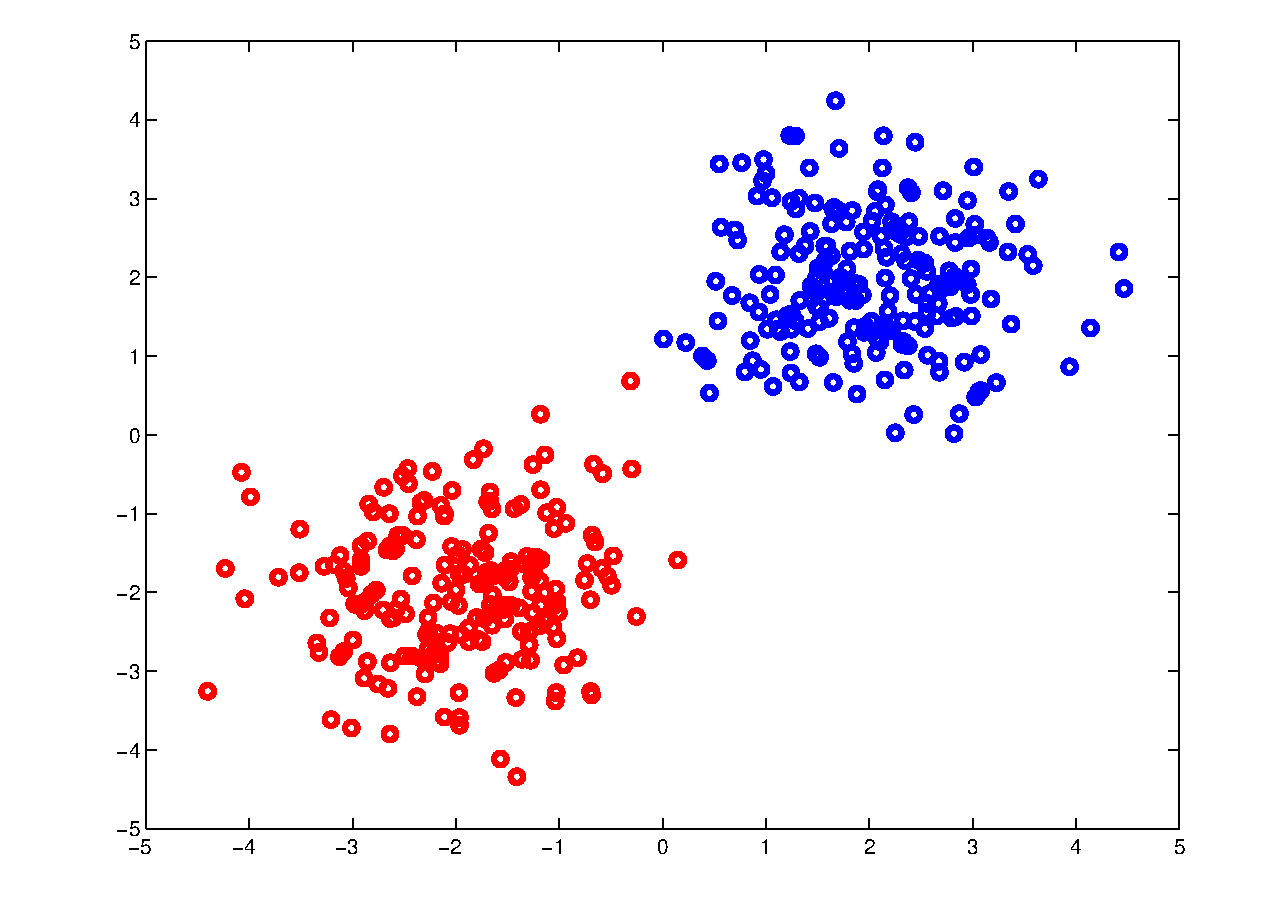
\includegraphics[width=0.45\columnwidth]{figures/linsep_data.pdf}
%    \label{fig:lisep_data}}
%     \subfloat[Linear boundary separating data.]
%     {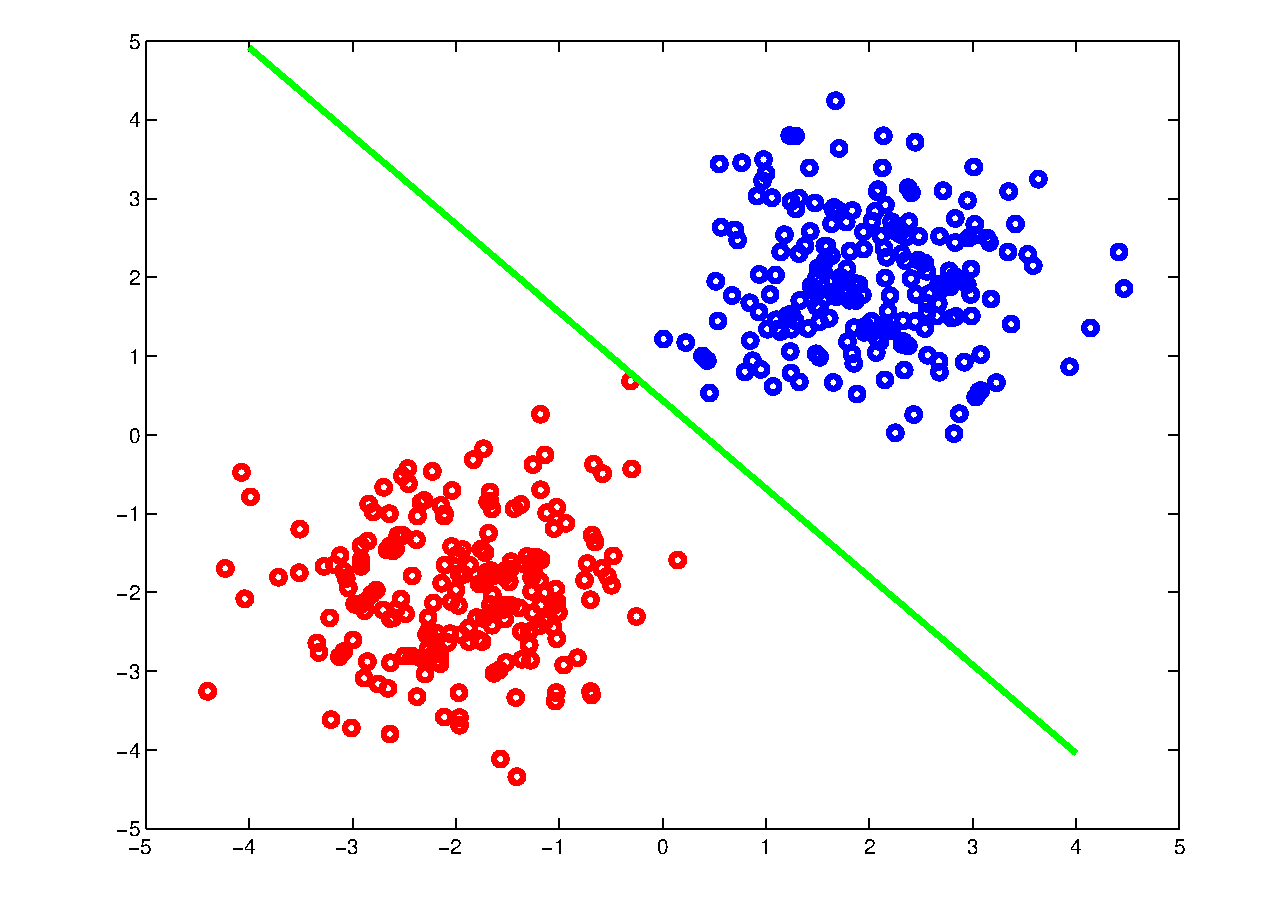
\includegraphics[width=0.45\columnwidth]{figures/linsep_data_perceptron.pdf}
%     \label{fig:lin_sep_bound}}  
%    \caption{Example of linearly separable data. Any simple linear learning algorithm e.g. perceptron, finds a solution.}
%    \label{fig:linsep}
%    %\end{figure}
%%\begin{figure}[tbh] %{r}{0.5\textwidth}
%\end{figure} 
%
%\begin{figure}
%\centering
%    \subfloat[Data from classes $A$ and $B$.]
%    {
%    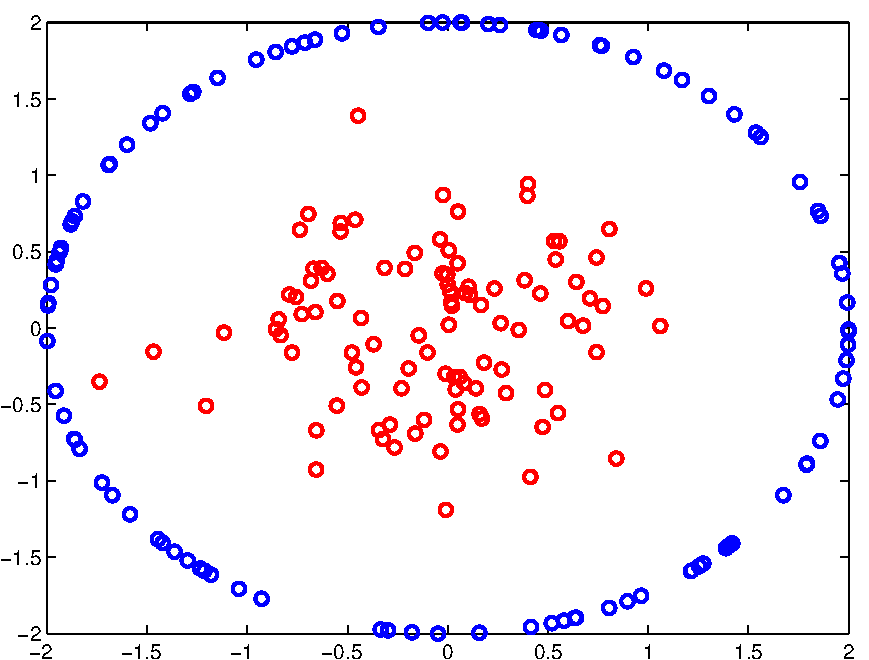
\includegraphics[width=0.45\columnwidth]{figures/pres_original_data.pdf}
%    \label{fig:nlisep_data}}
%     \[Linear boundary fails to separate data.]
%     {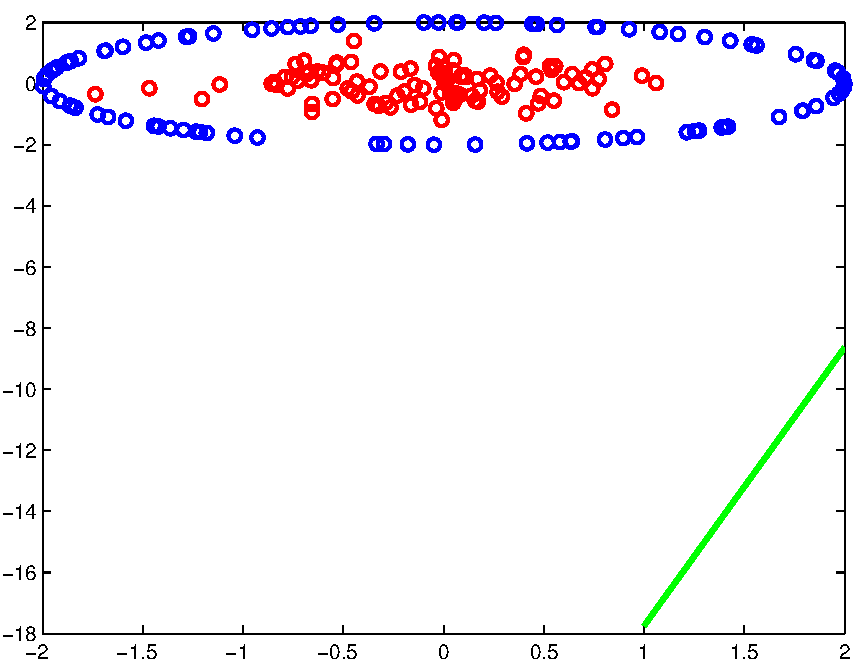
\includegraphics[width=0.45\columnwidth]{figures/pres_perc_original_data.pdf}
%     \label{fig:nlin_sep_bound}}  
%    \caption{Example of nonlinearly separable data. Perceptron fails to find a solution, and diverges.}
%    \label{fig:nlinsep}
%    %\end{figure}
%%\begin{figure}[tbh] %{r}{0.5\textwidth}
%\end{figure} 
%
%
%\begin{figure}
%\centering
%    \subfloat[Nonlinear mapping of data.]
%    {
%    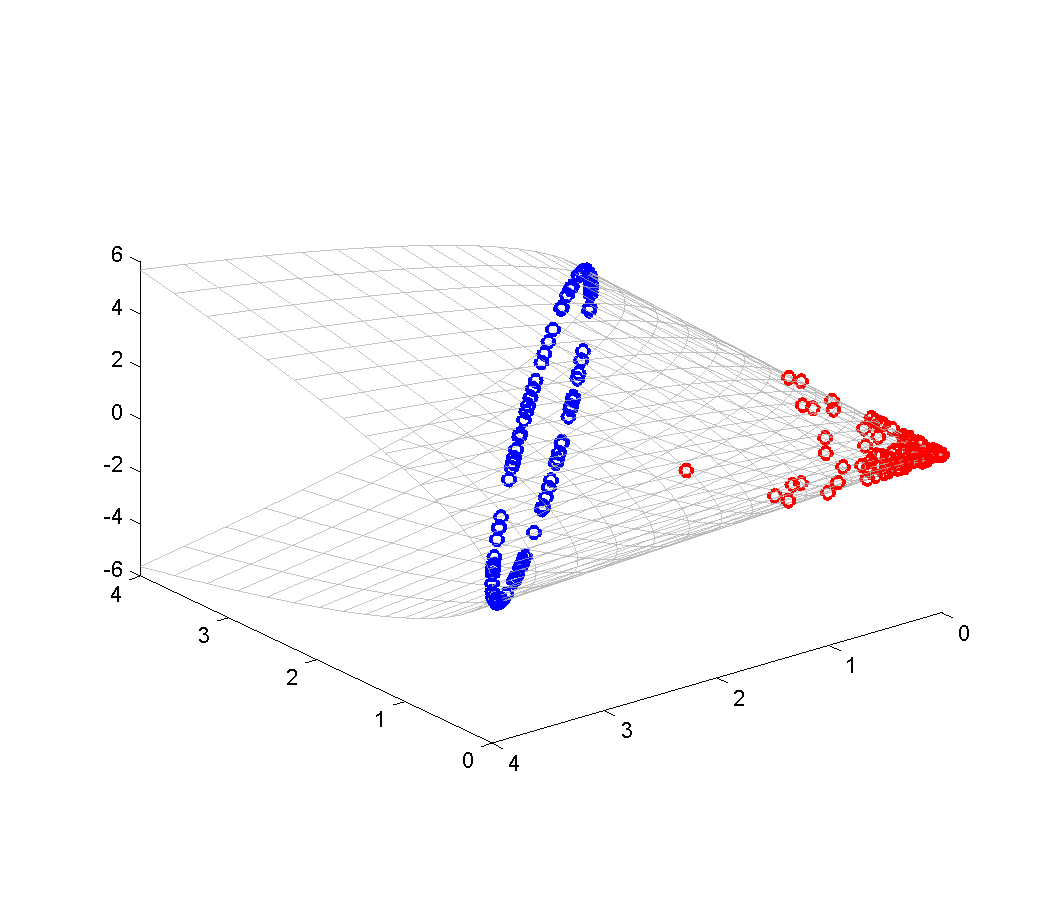
\includegraphics[width=0.45\columnwidth]{fmapped_data.pdf}
%    \label{fig:fmapped_data}}
%     \subfloat[Linear boundary in new space.]
%     {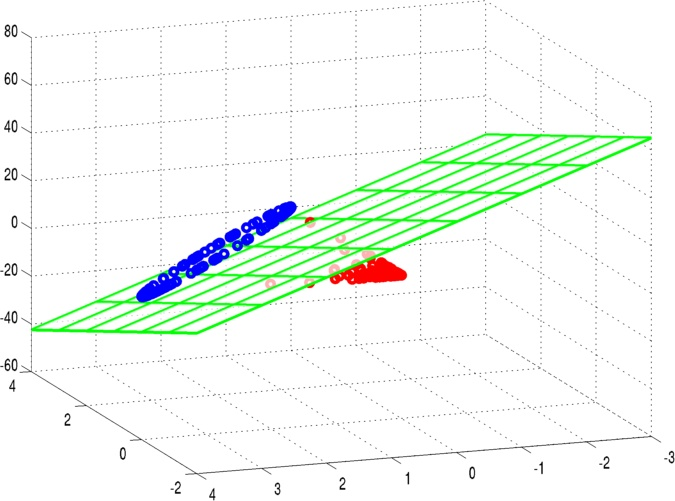
\includegraphics[width=0.45\columnwidth]{pres_perc_fmapped_data_after.jpg}
%     \label{fig:fmapped_bound}}  
%    \caption{If we map the same data using a nonlinear map $\phi(x,y):= (x^2, y^2, 2xy)$, the perceptron now finds a solution
%             in 3 dimensions.}
%    \label{fig:fmapped}
%    %\end{figure}
%%\begin{figure}[tbh] %{r}{0.5\textwidth}
%\end{figure} 